%%%%%%%%%%%%%%%%%%%%%%%%%%%%%%%%%%%%%%%%%%%%%%%%%%%%%%%%
\documentclass[10.5pt,a4paper]{article}% 文档格式
\usepackage{ctex,hyperref}% 输出汉字
% \usepackage{times}% 英文使用Times New Roman
%%%%%%%%%%%%%%%%%%%%%%%%%%%%%%%%%%%%%%%%%%%%%%%%%%%%%%%%

%%%%%%%%%%%%%%%%%%%%%%%%%%%%%%%%%%%%%%%%%%%%%%%%%%%%%%%%
\title{\fontsize{22pt}{20pt}\selectfont% 小四字号,1.5倍行距
	{\heiti% 黑体 
		关于深度学习优化算法的分析与实现}}% 题目
%%%%%%%%%%%%%%%%%%%%%%%%%%%%%%%%%%%%%%%%%%%%%%%%%%%%%%%%
\author{\fontsize{12pt}{12pt}\selectfont% 小四字号,1.5倍行距
	{\fangsong% 仿宋
		李志远}\\% 标题栏脚注
	\fontsize{10.5pt}{15.75pt}\selectfont% 小五字号,1.5倍行距
	{\fangsong% 仿宋
		(南京农业大学人工智能学院人工智能201 江苏 南京 210095)}}% 作者单位,“~”表示空格
%%%%%%%%%%%%%%%%%%%%%%%%%%%%%%%%%%%%%%%%%%%%%%%%%%%%%%%%
\date{}% 日期(这里避免生成日期)
%%%%%%%%%%%%%%%%%%%%%%%%%%%%%%%%%%%%%%%%%%%%%%%%%%%%%%%%
\usepackage{amsmath,amsfonts,amssymb}% 为公式输入创造条件的宏包
%%%%%%%%%%%%%%%%%%%%%%%%%%%%%%%%%%%%%%%%%%%%%%%%%%%%%%%%
\usepackage{graphicx}% 图片插入宏包
\usepackage{subfigure}% 并排子图
\usepackage{float}% 浮动环境,用于调整图片位置
\usepackage[export]{adjustbox}% 防止过宽的图片
%%%%%%%%%%%%%%%%%%%%%%%%%%%%%%%%%%%%%%%%%%%%%%%%%%%%%%%%
\usepackage{bibentry}
\usepackage{natbib}% 以上2个为参考文献宏包
%%%%%%%%%%%%%%%%%%%%%%%%%%%%%%%%%%%%%%%%%%%%%%%%%%%%%%%%
\usepackage{abstract}% 两栏文档,一栏摘要及关键字宏包
\renewcommand{\abstracttextfont}{\songti}% 摘要内容字体为宋体
%%%%%%%%%%%%%%%%%%%%%%%%%%%%%%%%%%%%%%%%%%%%%%%%%%%%%%%%
\usepackage[dvipsnames]{xcolor}% 字体颜色宏包
\newcommand{\red}[1]{\textcolor[rgb]{1.00,0.00,0.00}{#1}}
\newcommand{\blue}[1]{\textcolor[rgb]{0.00,0.00,1.00}{#1}}
\newcommand{\green}[1]{\textcolor[rgb]{0.00,1.00,0.00}{#1}}
\newcommand{\darkblue}[1]
{\textcolor[rgb]{0.00,0.00,0.50}{#1}}
\newcommand{\darkgreen}[1]
{\textcolor[rgb]{0.00,0.37,0.00}{#1}}
\newcommand{\darkred}[1]{\textcolor[rgb]{0.60,0.00,0.00}{#1}}
\newcommand{\brown}[1]{\textcolor[rgb]{0.50,0.30,0.00}{#1}}
\newcommand{\purple}[1]{\textcolor[rgb]{0.50,0.00,0.50}{#1}}% 为使用方便而编辑的新指令
%%%%%%%%%%%%%%%%%%%%%%%%%%%%%%%%%%%%%%%%%%%%%%%%%%%%%%%%
\usepackage{svg} % 插入svg图片
\usepackage{url}% 超链接
\usepackage{bm}% 加粗部分公式
\usepackage{multirow}
\usepackage{booktabs}
\usepackage{epstopdf}
\usepackage{epsfig}
\usepackage{longtable}% 长表格
\usepackage{supertabular}% 跨页表格
\usepackage{algorithm}
\usepackage{algorithmic}
\usepackage{changepage}% 换页
\usepackage{listings} % 代码
%%%%%%%%%%%%%%%%%%%%%%%%%%%%%%%%%%%%%%%%%%%%%%%%%%%%%%%%
\usepackage{tikz}
\tikzstyle{conv}=[rectangle, draw=black!80, fill=white!20, minimum size=2em]
\tikzstyle{add}=[rectangle, draw=black!80, fill=white!20, minimum size=2em]
\tikzstyle{group}=[rectangle, draw=black!80, fill=white!20, minimum size=2em]

%%%%%%%%%%%%%%%%%%%%%%%%%%%%%%%%%%%%%%%%%%%%%%%%%%%%%%%%
\usepackage{enumerate}% 短编号
\usepackage{caption}% 设置标题
\captionsetup[figure]{name=\fontsize{10pt}{15pt}\selectfont Figure}% 设置图片编号头
\captionsetup[table]{name=\fontsize{10pt}{15pt}\selectfont Table}% 设置表格编号头
%%%%%%%%%%%%%%%%%%%%%%%%%%%%%%%%%%%%%%%%%%%%%%%%%%%%%%%%
\usepackage{indentfirst}% 中文首行缩进
\usepackage[left=2.0cm,right=2.0cm,top=2.40cm,bottom=2.40cm]{geometry}% 页边距设置
\renewcommand{\baselinestretch}{1.5}% 定义行间距(1.5)
%%%%%%%%%%%%%%%%%%%%%%%%%%%%%%%%%%%%%%%%%%%%%%%%%%%%%%%%
\usepackage{fancyhdr} %设置全文页眉、页脚的格式
\pagestyle{fancy}
\hypersetup{colorlinks=true,linkcolor=black}% 去除引用红框,改变颜色
\lstset{   % 进行参数设置
 language=Python, % 设置语言
 basicstyle=\ttfamily, % 设置字体族
 breaklines=true, % 自动换行
 keywordstyle=\bfseries\color{NavyBlue}, % 设置关键字为粗体,颜色为 NavyBlue
 morekeywords={}, % 设置更多的关键字,用逗号分隔
 emph={self}, % 指定强调词,如果有多个,用逗号隔开
    emphstyle=\bfseries\color{Rhodamine}, % 强调词样式设置
    commentstyle=\itshape\color{black!50!white}, % 设置注释样式,斜体,浅灰色
    stringstyle=\bfseries\color{PineGreen!90!black}, % 设置字符串样式
    columns=flexible
} 
%%%%%%%%%%%%%%%%%%%%%%%%%%%%%%%%%%%%%%%%%%%%%%%%%%%%%%%%

\begin{document}% 以下为正文内容
	\maketitle% 产生标题,没有它无法显示标题
	%%%%%%%%%%%%%%%%%%%%%%%%%%%%%%%%%%%%%%%%%%%%%%%%%%%%%%%%
	\lhead{}% 页眉左边设为空
	\chead{}% 页眉中间设为空
	\rhead{}% 页眉右边设为空
	\lfoot{}% 页脚左边设为空
	\cfoot{\thepage}% 页脚中间显示页码
	\rfoot{}% 页脚右边设为空
	%%%%%%%%%%%%%%%%%%%%%%%%%%%%%%%%%%%%%%%%%%%%%%%%%%%%%%%%
	\begin{adjustwidth}{1.06cm}{1.06cm}
            \fontsize{9pt}{13.5pt}\heiti{摘要:}\songti 本文旨在深入了解深度学习中的优化算法,掌握其原理、特点以及超参数的调整等方面知识,并进行实验验证。我选择了一篇深度学习优化算法综述\cite{zongshu}与动手学深度学习\cite{d2l}的部分章节作为参考资料。在这些资料的基础上,我动手实现了大部分优化算法,并使用自定义网络和Fashion-MNIST数据集进行了实验验证。实验结果表明,使用不同的优化算法对于训练神经网络的性能和训练时间都有显著的影响,不同的优化算法在不同的数据集和网络结构中表现得也不尽相同,因此选择合适的优化算法和设置合适的超参数对于深度学习的实际应用非常重要。通过对优化算法的深入了解,我们能够更有针对性地选择优化算法,并更加精准地进行超参数的调整,从而提高模型训练效率和性能。
	\end{adjustwidth}
	\begin{adjustwidth}{1.06cm}{1.06cm}
		\fontsize{9pt}{10pt}\selectfont{\heiti{关键词:}\songti{深度学习;优化算法;梯度下降}}\\
	\end{adjustwidth}

	\begin{adjustwidth}{1.06cm}{1.06cm}% 英文摘要内容
		\fontsize{9pt}{10pt}\selectfont{\heiti{\textbf{Abstract:}}\songti{This paper aims to understand the optimization algorithm in deep learning, master its principle, characteristics and hyperparameter tuning, and carry out experimental verification. I chose a survey on Deep Learning Optimization Algorithms and parts of Hands-on Deep Learning as references. On the basis of these materials, I manually implemented most of the optimization algorithms and carried out experimental verification using custom networks and Fashion-MNIST dataset. The experimental results show that the use of different optimization algorithms has a significant impact on the performance and training time of neural networks, and different optimization algorithms perform differently in different datasets and network structures. Therefore, choosing the appropriate optimization algorithm and  hyperparameters are very important for the practical application of deep learning. Through a deep understanding of the optimization algorithm, we can choose the optimization algorithm more pertinently, and tune the hyperparameters more accurately, so as to improve the training efficiency and performance of the model. }}
	\end{adjustwidth}
         \begin{adjustwidth}{1.06cm}{1.06cm}
		\fontsize{9pt}{10pt}\selectfont{\heiti{\textbf{Keywords:}}\songti{Deep Learning;Optimization;Gradient Descent}}\\
	\end{adjustwidth}
	\newpage% 从新的一页继续
        \section{导言}
        优化算法对于深度学习非常重要,优化算法决定了我们以什么样的方式更新模型参数,从而能够达到目标函数最小化的目的,然而在日常的使用当中,我们大多数时间仅仅是将其作为“炼丹”的一种药材,停留在一知半解的程度。因此在本次课程设计当中,我略读了大量的优化算法文献,精读一篇深度学习优化算法综述\cite{zongshu}与动手学深度学习\cite{d2l}关于优化算法的部分,以理解并分析算法原理为目的,动手实现了大部分算法并使用自定义网络与FashionMNIST数据集进行了实验验证。\par
        训练较为复杂、深或宽的神经网络往往需要数小时、数天甚至数周,其中优化算法的性能将会直接影响到模型的训练效率,当模型通过反向传播计算梯度结束后,要使用优化算法来将模型参数作优化,就需要对整个模型参数进行修改;尽管参数更新的耗时不如前向传播与反向传播占比大,但时间快只是目标的一部分,对其进行改进仍然是深度学习重要的任务之一。\par
        在对优化算法进行了解后,在训练网络时对于其的选择不再是一个抽奖环节,而是更能有针对性的选择适合的优化算法进行训练;同时对于优化算法中的超参数设置也有了一定的理解,使我们能够在调整超参数时更加有针对性,已达到提升模型训练效率、提升模型性能的目的。\par
        \section{基本设置}
        在开始介绍优化算法之前,我们先将所用到的参数作一个统一的说明,同时本次实验使用的网络以及数据集做一个简短的介绍,以在介绍算法时展示该优化算法下的模型性能。
        \subsection{数据集}
        本次试验使用FashionMNIST数据集\cite{fashionmnist},该数据集包括10个类别、70000张图片,每个类别含7000张,每张图片大小为$28\times28$,训练集有60000张图片,测试集有10000张。由于我们的目的是比较优化算法的效果,因此不对数据集作增强处理。
        \subsection{模型}
        模型使用CNN架构,细节如下:三层卷积层,通道数分别为[72, 256, 128],卷积核大小均为$3\times3$,每层卷积后均有batchnorm、ReLU、maxpool层;一层$128\times84$的线性层、BatchNorm层、ReLU,再接一层$84\times10$的分类层。
        \begin{figure}[h]
            \includesvg[width=\textwidth]{nn.svg}
            \caption{模型结构简图}
        \end{figure}
        \subsection{参数说明}
        对基本的参数做一个说明,在具体到每一个优化算法当中独有的参数会在算法当中解释。
        \begin{itemize}
            \item $J(\theta)\qquad \theta\in\mathbb{R}^d$: 目标函数
            \item $\theta: \mathbb{R}^d$: d维模型参数
            \item $\nabla_\theta J(\theta)$: 目标函数关于参数$\theta$的梯度
            \item $t$: 时间步(step)
        \end{itemize}
        \subsection{优化器的基本设置}
        由于从0开始实现不能很好的融入深度学习训练框架,我继承了torch的优化器基类Optimizer,这样的优点是优化器基本的参数获取、超参数等设置都有一个接口,同时zero\_grad()方法也能够直接使用,事实上前面提到的不能很好的融入的原因就是在我手写的zero\_grad()方法中将梯度设置为0后参数迭代器就不可用了,才使用了基类继承的方式。\par
        虽然不算作从0开始实现,但算法的关键:更新操作还是从0开始的,每个算法的细节将会在每一小节进行详细的说明。\par
        在Optimizer类中,参数放入名为param\_groups中,每一个参数都以字典的形式将超参数与自己关联起来,这在一些例如微调模型中将起到作用,对于本实验没有影响,因此我们沿用了这种形式,将超参数统一作为字典接受。以能够使框架适配所有优化算法\par
        \subsection{超参数设置}
        在介绍之前,将统一设置的超参数的值作一个说明,在每个小节中,若无额外说明,则均采用如下所需的超参数:
        \begin{table}[!ht]
        \centering
        \begin{tabular}{|l|l|l|}
        \hline
            超参数 & 值 & 优化算法\\ \hline
            learning rate & 0.01 & all\\ \hline
            momentum & 0.9 & SGD with momentum\\ \hline
            nesterov & True & SGD with momentum\\ \hline
            batch size & 256 & all \\ \hline
            epochs & 5 & all\\ \hline
        \end{tabular}
        \caption{超参数设置}
         \end{table}\par
         在训练时能够明显的看出我们的模型还没有拟合,这是因为我们需要关注优化算法的收敛性能,而不是最终模型的效果,因此需要注重前期的收敛速度以及损失的值,事实上,我们为每个模型训练了25个epoch,训练结果图将在附录中给出。
        \section{梯度下降}
        梯度下降目前已经很少直接用于优化目标函数,我们在深度学习框架当中使用较多的SGD实质上是MBSGD(mini-batch stochastic gradient descent),即小批量随机梯度下降,其已经集成了梯度下降较多的优化策略,例如动量、Nesterov等等,在本部分中,我们将对基于SGD的优化算法作一个分析与说明,并对后三者进行实现,不对其余两算法进行实现的原因将在小节内说明。
        \subsection{批量梯度下降(BGD)}
            在本节中,我们首先对梯度下降的原理,即梯度下降为何能够使目标函数值减小作一个数学上的说明,考虑目标函数$J(\theta): \mathbb{R}^d\to\mathbb{R}$、模型参数$\theta$的一阶泰勒展开:
            \begin{align*}
                J(\mathbf{\theta}+\epsilon)=J(\mathbf{\theta})+\epsilon^{\top}\nabla J(\mathbf{\theta})+\mathcal{O}(\|\epsilon\|^2)
            \end{align*}
            我们可以通过当前函数值与梯度来确定$J(\mathbf{\theta}+\epsilon)$的值,当我们选择合适的$\epsilon$时,就可能能够使$J$的值减小。具体地说,选择固定步长$\eta\ge 0$, 然后取$\epsilon=-\eta\nabla J(\mathbf{\theta})$代入上式,我们得到
            \begin{align*}
                J(\mathbf{\theta}-\eta\nabla J(\mathbf{\theta}))=J(\mathbf{\theta})-\eta\|\nabla J(\mathbf{\theta})\|^2+\mathcal{O}(\|\epsilon\|^2)
            \end{align*}
            这意味着如果我们使用$\mathbf{\theta}\gets\mathbf{\theta}-\eta\nabla J(\mathbf{\theta})$来迭代$\mathbf{\theta}$,函数值可能会减小,这就是梯度下降为什么能够使函数值减小的原因。\par
            梯度下降算法的思想来源于1951年发表的一篇文章\cite{sgd},文章希望找到方程$M(x) = \alpha$的解$x = \theta$,其中$\alpha$是给定常数。其给出了一种在第$x_1,x_2,\cdots,x_n$级进行连续实验的方法,使$x_n$在概率上趋向于$\theta$。当$\alpha=0$时,该算法得出的迭代方式即为梯度下降的方式。\par
            批量梯度下降即每次利用整个训练集的数据更新模型参数,每个周期只进行一次更新,其更新方式如下:
            \begin{align*}
                \theta = \theta-\eta\,\cdot\,\nabla_\theta J(\theta)
            \end{align*}
            由于一次采用整个训练集来更新参数,批量梯度下降能够保证模型收敛于局部最小值;但这种只进行一次更新,在整个数据集上进行计算的方式要求的环境十分苛刻,首先如果数据集的量级达到一定程度的话,主存或GPU的内存很有可能会不足从而不能达到目的.
        \subsection{随机梯度下降(SGD)}
            在批量梯度下降中,我们一次选取整个数据集的数据进行损失的计算,其缺点很明显,而随机梯度下降则是另一个极端:它每次更新只随机选择一个样本计算梯度更新参数,其更新方式如下:
            \begin{align*}
                \theta=\theta-\eta\cdot\nabla_\theta J(\theta;x^{(i)};y^{(i)})
            \end{align*}
            其中$x^{(i)}$为样本,$y^{(i)}$为样本对应的标签。由于加入的是一个随机变量而不是之前的均值,变量的更新变得没那么稳定,即使函数已经接近极小值的情况下,仍然有可能因为随机变量的不确定性导致较大的梯度更新,从而引发函数值振荡;然而这种振荡带来的好处是函数可能会进入新的更好的局部最小值,我们可以通过设置动态学习率的方法来缓解函数在局部最优点附近的振荡。随机梯度下降相比于批量梯度下降最大的优势在于其将每次更新的计算复杂度从$O(n)$降为了$O(1)$,n表示数据集大小。
            在实现当中,由于我在网络设置当中增添了BN层,因此不能设置batch\_size为1,我们使用batch\_size为2进行代替,此处仅展示结果,在下一小节一并说明算法的细节。
            \begin{figure}[H]
            \centering
                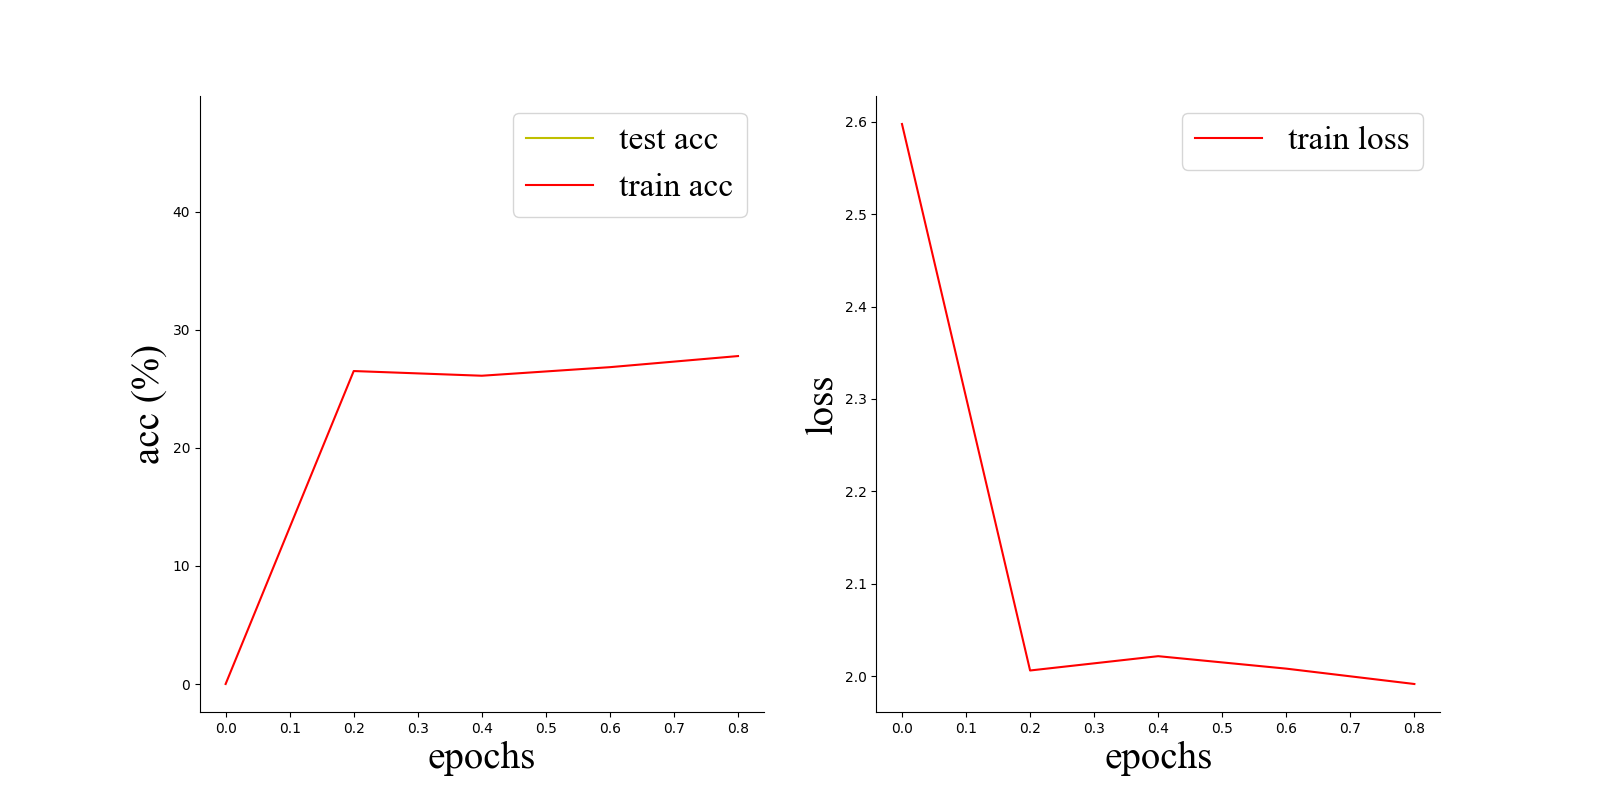
\includegraphics[width=0.8\textwidth]{SGD_batch_2.png}
              \caption{SGD batch\_size=2的训练结果}
              \label{fig:SGD}
            \end{figure}
            由于其训练效率实在太低,我们仅训练了1个epoch,其运算速度约为200 examples/sec,是其余算法的1/65。测试准确率约为47\%,在多个epoch的情况下准确率还会提升,但其代价太大,我们仅展示该训练结果。
        \subsection{小批量随机梯度下降(MBSGD)}
            在梯度下降方法中,批量梯度下降在每次计算高昂的复杂度使其不那么常用;随机梯度下降由于无法利用GPU并行计算的优势,在实际使用中耗费时间往往会很久。小批量随机梯度下降即为综合考虑两者的优点而选择的方案。
            小批量计算得到的梯度在更新时参与计算的是小批量梯度的均值,对于梯度的统计属性而言,均值与原来相同,方差减小,能够在收敛时更加稳定;同时提供了并行性,能够使用GPU以及当前深度学习库加速计算,具体而言,其更新方式如下:
            \begin{align*}
                \theta=\theta-\eta\cdot\nabla_\theta J(\theta;x^{(i:i+n)};y^{(i:i+n)})
            \end{align*}
            其中$x^{(i:i+n)};y^{(i:i+n)}$为n个小批量的样本与标签。
            \subsubsection{实现}
            事实上,我们实现小批量随机梯度下降直接每次更新时将参数减去学习率与参数梯度的乘积即可,本质只需一行代码:
            \begin{lstlisting}[language=python]
            p2.data.sub_(p1['lr'] * p2.grad)
            \end{lstlisting}
\newpage
            实验结果如下:
            \begin{figure}[H]
            \centering
                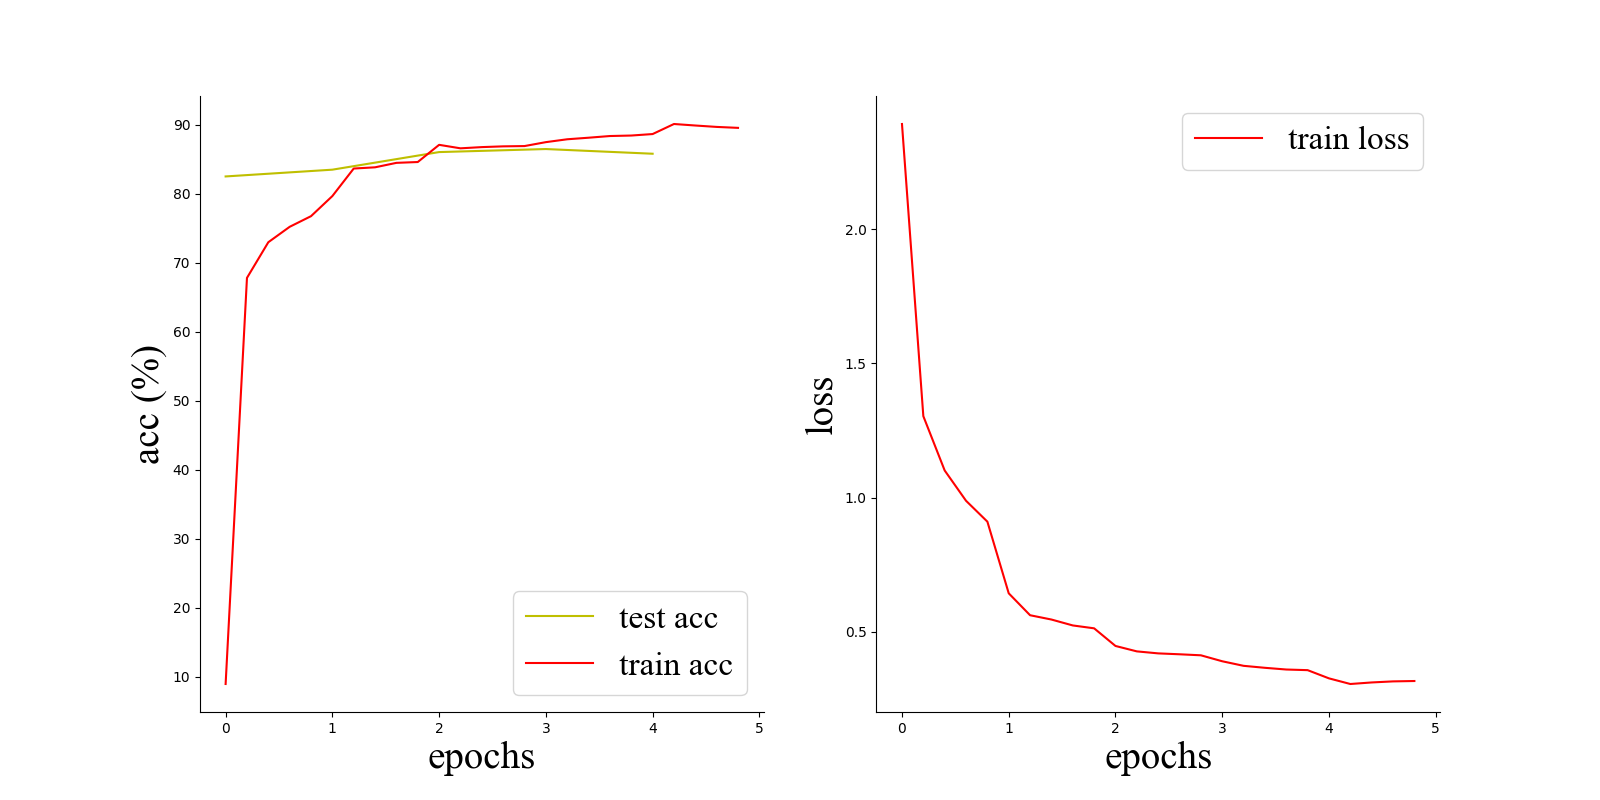
\includegraphics[width=0.8\textwidth]{imgs_5e/SGD.png}
              \caption{MBSGD的训练结果}
              \label{fig:SGD}
            \end{figure}  
            经过5个epoch的训练,模型在训练集上的准确率为0.896,测试集上的准确率为0.858,损失函数值为0.317,训练速度为11670.2 examples/sec on cuda:0。\par
            与批量梯度下降算法相比,小批量随机梯度下降的训练速度更快,但是随机性也带来了一定的噪声和不稳定性,导致收敛过程可能不够平滑。然而,这种随机性使随机梯度下降还可以避免陷入局部最优解,因为每次选择的小批量样本是随机的,模型会在参数空间中不断跳跃,从而有更多的机会发现全局最优解。\par
            事实上,在小批量随机梯度下降中分别取batch\_size=1与n即为随机梯度下降与批量梯度下降,由于在网络中设置了BN层因此不能取1,而n(数据集大小)在实验所用数据集使用会导致内存不足,因此没有对前两个算法进行详细的实现。
        \subsection{动量随机梯度下降(SGD with momentum)}
            动量随机梯度下降\cite{momentum}是一种基于梯度的优化算法,它通过加入动量项来抑制随机梯度下降(SGD)算法在局部最优值附近发生的震荡现象,加速收敛速度。动量算法的更新规则如下:
            \begin{align*}
                \begin{array}{l}v_t=\gamma v_{t-1}+\eta\nabla_\theta J(\theta)\\ \theta=\theta-v_t\end{array}
            \end{align*}
            其中$v$为我们的累计梯度,动量算法在每次迭代时,将上一次更新的向量的一部分(即动量项)与本次更新的向量相加,来确定下一次的更新方向和大小。这样可以让模型参数在梯度方向上累积动量,使更新方向更加稳定。\par
            动量算法中的动量系数$\gamma$通常取0.9,这个值可以调整,但一般情况下不需要进行太多的调整。$\gamma$越大,更新时就会保留更多的历史信息,使得更新方向更加稳定,但也可能会导致更新过程过于平滑而错过更好的解。相反,$\gamma$越小,更新方向更加灵活,但也更容易受到噪声的影响。
\newpage
            \subsubsection{实现}
            我们需要维护一个向量v,用于存储过去梯度的累积,其更新代码如下:
            \begin{lstlisting}
                v[:] = p1['momentum'] * v + p1['lr'] * p2.grad
                p2[:] -= v
            \end{lstlisting}\par
            实验结果如下:
            \begin{figure}[H]
            \centering
                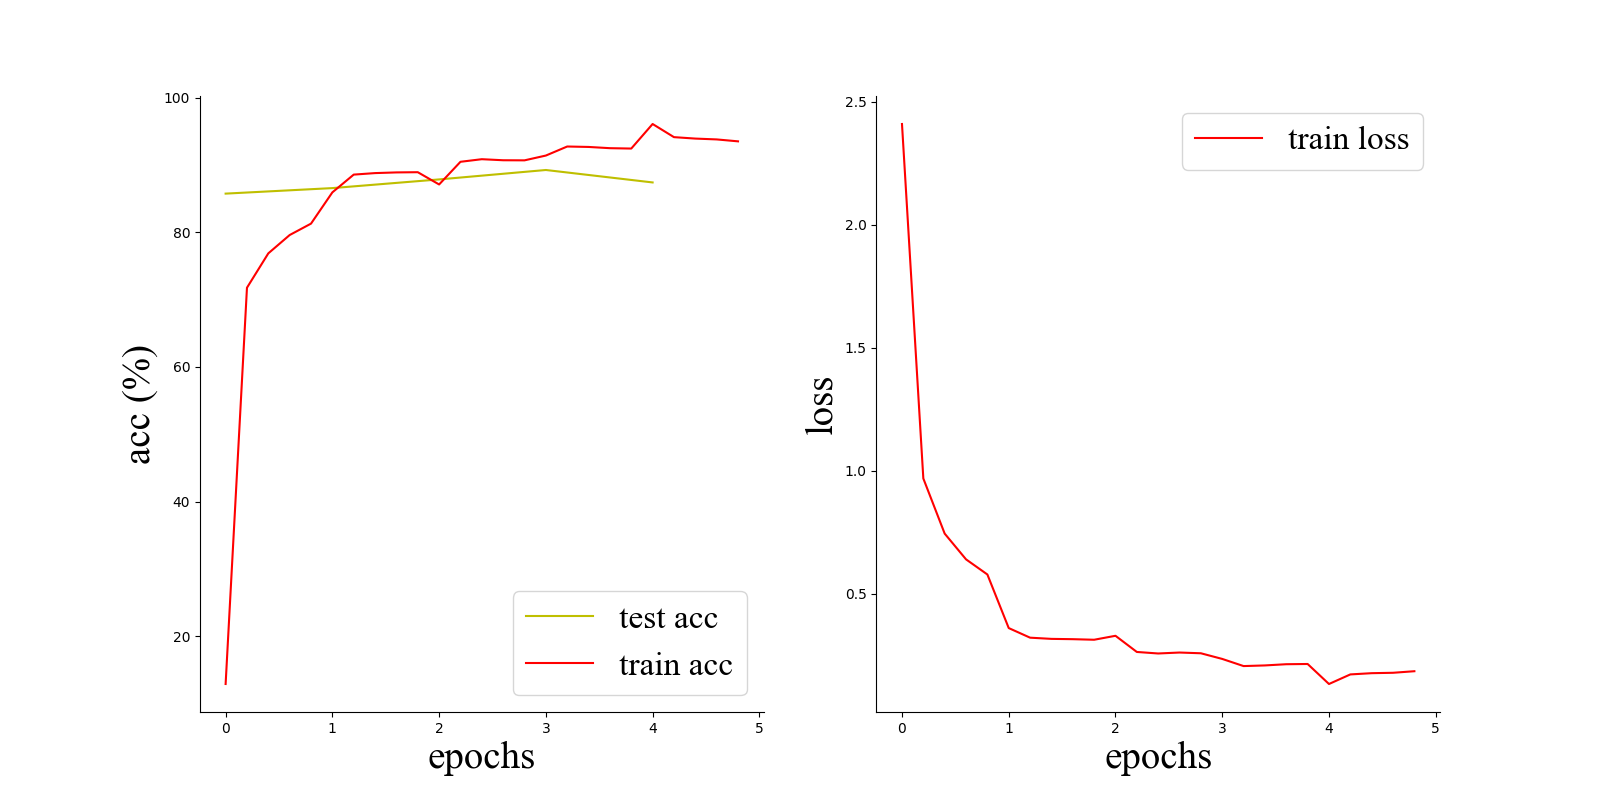
\includegraphics[width=0.8\textwidth]{imgs_5e/SGD_momentum.png}
              \caption{SGD\_momentum的训练结果}
              \label{fig:SGD_m}
            \end{figure} 
            经过5个epoch的训练,模型在训练集上的准确率为0.935,测试集上的准确率为0.874,损失函数值为0.184,训练速度为12973.0 examples/sec on cuda:0。\par
            由实验结果可以看出,momentum的加速效果还是比较明显的,loss前期下降的更快一些,训练集准确率也更高。
        \subsection{NAG}
            nesterov加速梯度\cite{nagsgd}算法通过在动量方法中给参数一个下一时刻的近似位置,来更准确地计算梯度,进而加速SGD的速度。具体实现方式是先更新动量,然后在近似位置上计算梯度,并使用更新后的动量更新参数。具体方式如下:
            \begin{align*}
                \begin{array}{l}v_t=\gamma v_{t-1}+\eta\nabla_\theta J(\theta-\gamma v_{t-1})\\ \theta=\theta-v_t\end{array}
            \end{align*}
            通过该算法可以根据误差函数的梯度调整更新从而进一步加速SGD。
            \subsubsection{实现}
            在实际实现上,我们基于动量法的公式将$\nabla_\theta J(\theta-\gamma v_{t-1})\text{中的}v_{t-1}$改变一下更新时间,将算法调整为
            \begin{align*}
                \begin{array}{l}v_t=\gamma v_{t-1}+\eta\nabla_\theta J(\theta)\\ \theta=\theta-v_t-\gamma v_{t}\end{array}
            \end{align*}
            如果不这样改变,意味着我们要在优化算法开始之前先更新模型的参数,这显然是不合理的,综上所述,更新的关键代码为:
            \begin{lstlisting}
                v[:] = p1['momentum'] * v + p1['lr'] * p2.grad
                p2[:] -= (1 + p1['momentum']) * v
            \end{lstlisting}\par
            实验结果如下:
            \begin{figure}[H]
            \centering
                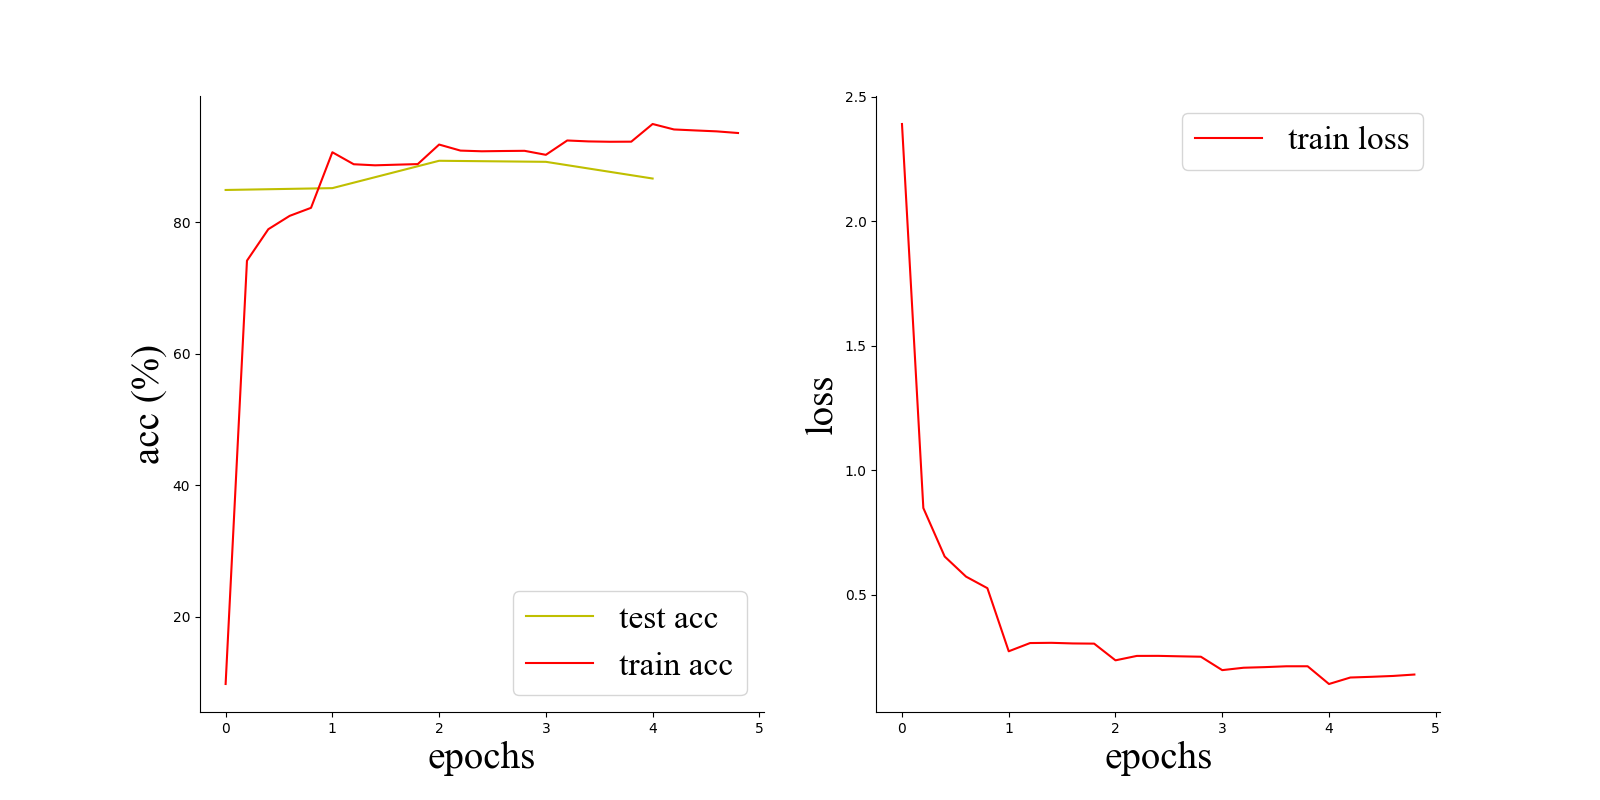
\includegraphics[width=0.8\textwidth]{imgs_5e/SGD_momentum_nesterov.png}
              \caption{SGD\_momentum\_nesterov的训练结果}
              \label{fig:SGD_m_n}
            \end{figure} 
            最终,经过5个epoch的训练,得到的损失函数值为0.179,训练集和测试集上的准确率分别为0.936和0.866,训练速度为12829.4 examples/sec on cuda:0。\par
            虽然不太明显,但结果也验证了NAG确实会比动量法更快一些。
        \section{自适应学习率}
        自适应学习率优化算法是一类基于梯度信息自适应地调整学习率的优化算法。与传统的优化算法不同,它不需要手动调节学习率,而是根据每个参数的梯度信息动态地调整学习率。这样可以使得算法更加适应不同的参数空间,从而提高模型的性能。常见的自适应学习率优化算法有AdaGrad、RMSProp、AdaDelta、Adam等。本部分我们将对其一一说明并实现。
        \subsection{AdaGrad}
            Adagrad\cite{adagrad}能够根据参数动态调整学习率,对低频出现的参数执行较大更新,对高频出现的参数执行较小的更新。\par
            先前我们进行一次更新时,对每一个参数$\theta_i$都使用相同的学习率$\eta$,而Adagrad时间步不同、参数不同则学习率也不同,因此我们定义$g_{t,i}$为目标函数关于时间步$t$和参数$\theta_i$的梯度,即
            $$g_{t,i}=\nabla_{\theta_t}J(\theta_{t,i})$$
            更新方式为
            $$\theta_{t+1,i}=\theta_{t,i}-\dfrac{\eta}{\sqrt{G_{t,ii}+\epsilon}}\cdot g_{t,i}$$
            其中$G_t\in\mathbb{R}^{d\times d}$ 是一个对角阵,对角线上第i个值为第i个参数从开始到t个时间步的梯度的平方和,即$G_{t,ii}=\Sigma_{j=1}^tg_{j,i}^2\quad\qquad i=1,2,\cdots,d$。$\epsilon$是一个极小量,避免分母为0,将更新方式写为向量形式,即
            \begin{align*}
            \theta_{t+1}=\theta_t-\dfrac{\eta}{\sqrt{G_t+\epsilon}}\odot g_t 
            \end{align*}\par
            Adagrad最大的优点是他不需要再手动的调整学习率,大多数实现都使用默认值0.01,缺点是G的累积都是正值,其和在训练过程中不断增长,最终学习率会变得无穷小,导致算法不能进行更新。
            \subsubsection{实现}
            我们需要维护一个变量G,用来存储过去梯度的平方累积,其更新的关键代码如下:
            \begin{lstlisting}
                g_tii[:] += torch.square(p2.grad)
                p2[:] -= p1['lr'] * p2.grad / torch.sqrt(g_tii + epsilon)
            \end{lstlisting}\par
            实验结果如下:
            \begin{figure}[H]
            \centering
                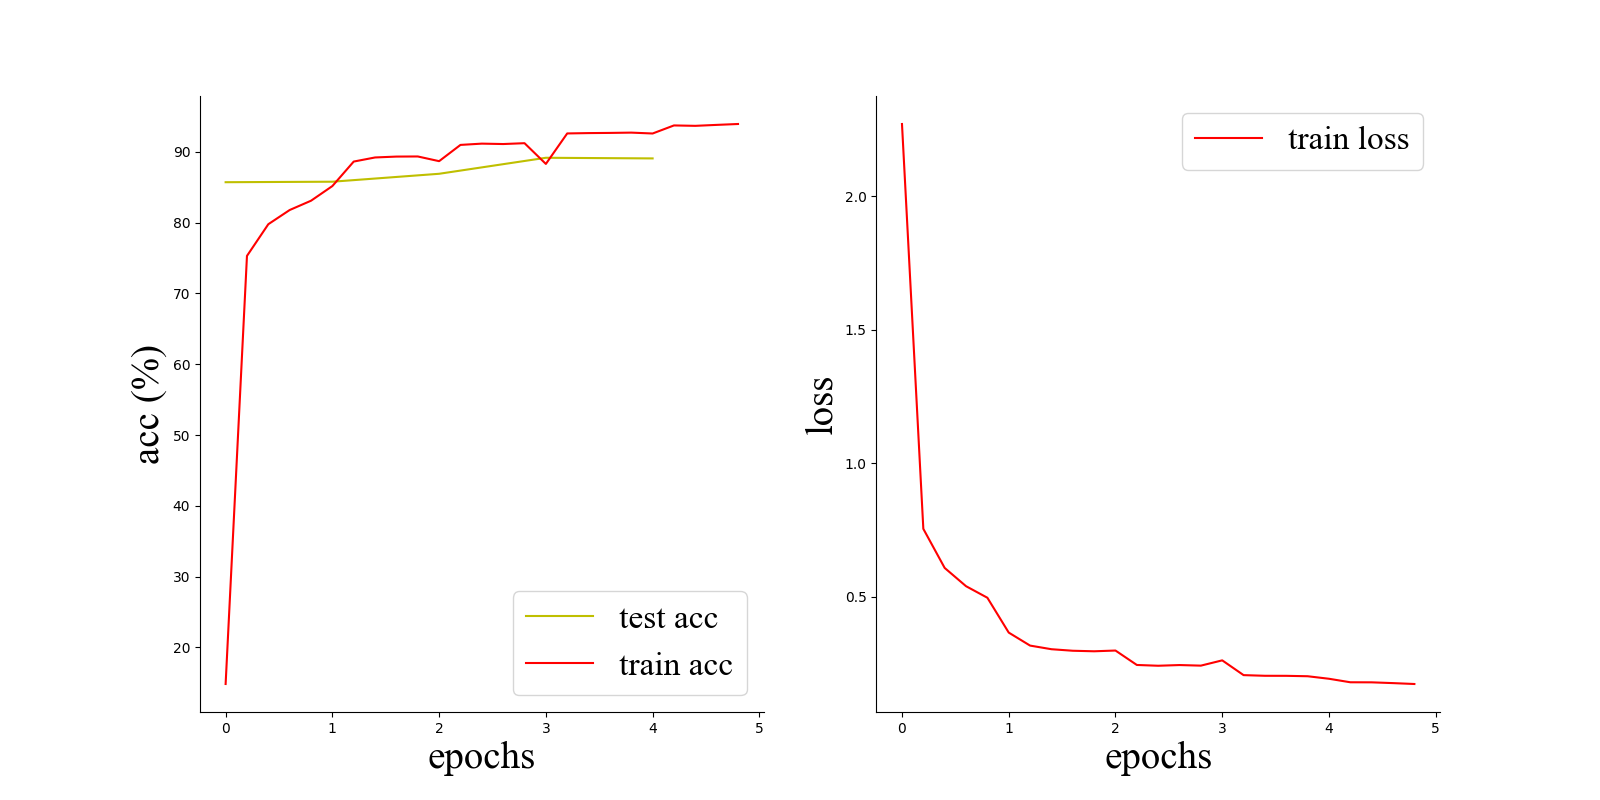
\includegraphics[width=0.8\textwidth]{imgs_5e/AdaGrad.png}
              \caption{AdaGrad的训练结果}
              \label{fig:adagrad}
            \end{figure} 
            最终,经过5个epoch的训练,得到的损失函数值为0.174,训练集和测试集上的准确率分别为0.939和0.891,训练速度为12690.4 examples/sec on cuda:0。\par
            尽管其缺点很明显,自适应学习率的先天优势仍然能够使其比SGD系列最快的损失函数值要更低;然而其缺点也在之后的方法中被成功修正。
        \subsection{RMSProp}
            RMSProp全称为Root Mean Square Propagation,是一种常见的自适应学习率优化算法,由Hinton在Coursera上的课程中提出。\par
            RMSProp的基本思想是在更新参数时,对梯度进行平方加权平均,并将其除以加权平均平方根和一个小常数(为了避免分母为0),得到的结果即为调整后的学习率。RMSProp的更新公式为:
            \begin{align*}E[g^2]_t&=0.9E[g^2]_{t-1}+0.1g^2_t\\ \theta_{t+1}&=\theta_t-\frac{\eta}{\sqrt{E[g^2]_t+\epsilon}}g_t
            \end{align*}
		其中$E[g^2]_t$为梯度平方的指数加权平均,RMSProp的优点是对梯度进行了平滑处理,可以减少梯度的波动,从而在收敛过程中更加稳定。由于RMSProp与AdaDelta较为相似,我们会在下一小节详细说明算法的细节。
            \subsubsection{实现}
            我们维护变量E\_g来存储梯度平方的指数衰减平均,代码如下:
            \begin{lstlisting}
                Eg_t[:] = 0.9 * Eg_t + 0.1 * torch.square(p2.grad)
                p2[:] -= p1['lr'] * p2.grad / torch.sqrt(Eg_t + epsilon)
            \end{lstlisting}\par
            实验结果如下:
            \begin{figure}[H]
            \centering
                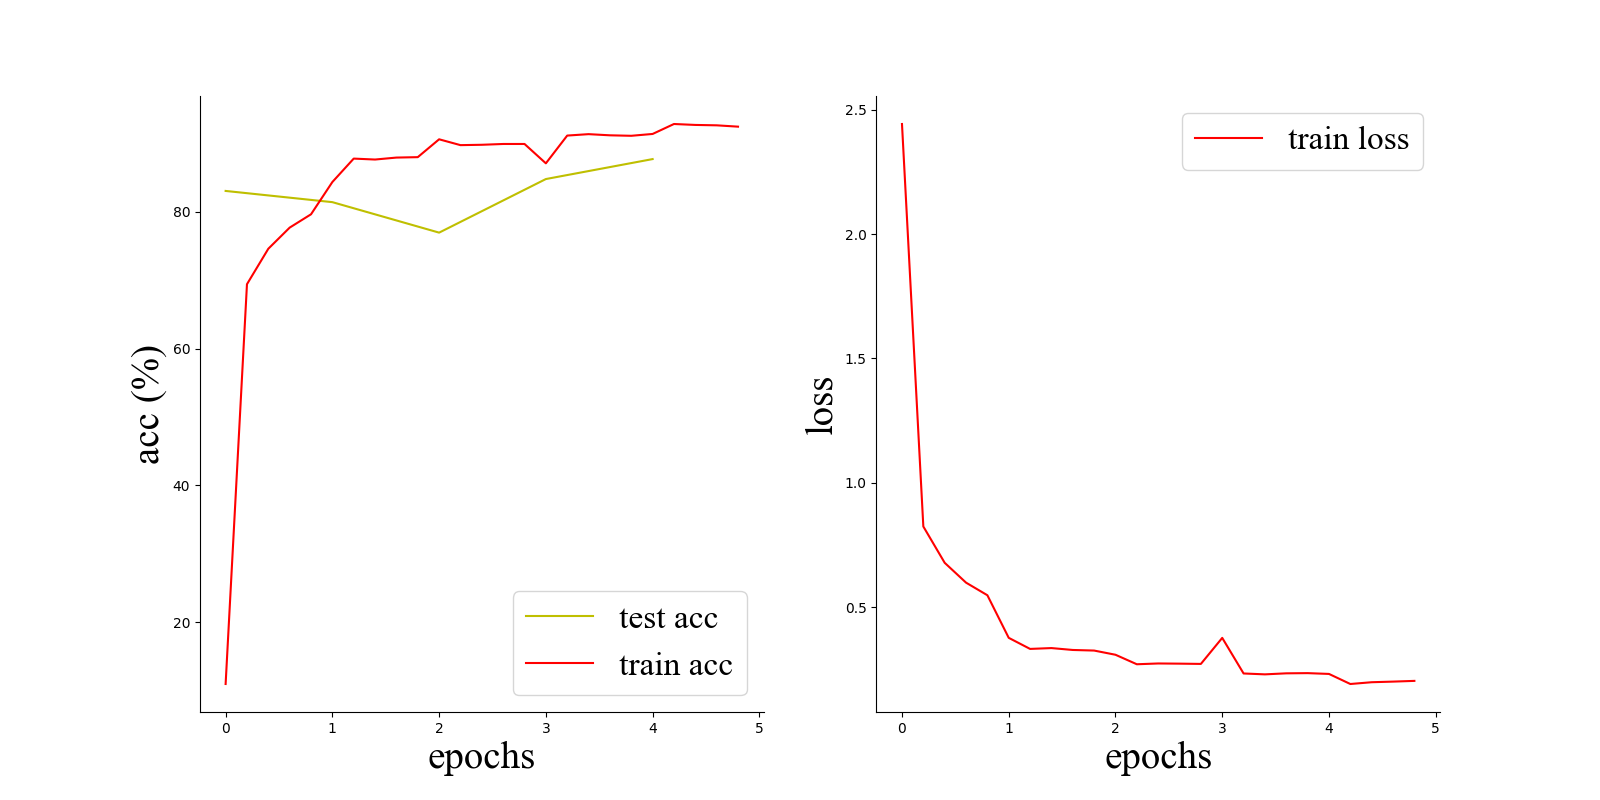
\includegraphics[width=0.8\textwidth]{imgs_5e/RMSProp.png}
              \caption{RMSProp的训练结果}
              \label{fig:rmsprop}
            \end{figure} 
            最终,经过5个epoch的训练,得到的损失函数值为0.204,训练集和测试集上的准确率分别为0.925和0.877,训练速度为12275.3 examples/sec on cuda:0。\par
        \subsection{AdaDelta}
            在AdaGrad中曾提到其缺点是梯度平方G的累积都是正值,其和在训练过程中不断增长,最终学习率会变得无穷小,导致算法不能进行更新。Adadelta\cite{adadelta}会控制积累过去梯度的大小,不会无限制的积累,从而避免学习率无穷小的问题。\textbf{窗口大小由t变为一个固定的w,即每次只看(累加)前面w步的梯度,而不是所有梯度都看;而储存w个梯度是低效的,实现变成了计算衰减平均。}确切的说,梯度和被递归定义为过去所有平方梯度的衰减平均值,t时刻的平均值仅依赖于$\gamma$倍的之前的平均值和当前梯度
            $$E[g^2]_t=\gamma E[g^2]_{t-1}+(1-\gamma)g_t^2$$
            只需要把Adagrad向量更新公式中的$G_t$换为$E[g^2]_{t-1}$,就得到了Adadelta的更新公式,即
            $$ \Delta\theta_t=-\dfrac{\eta}{\sqrt{E[g^2]_t+\epsilon}}g_t$$
            其中分母是梯度的均方根(RMS)误差准则,我们将其简写为$\Delta\theta_t=-\dfrac{\eta}{RMS[g]_t}g_t$。\par
            作者指出,此更新中的单位(以及SGD、Momentum或Adagrad)不匹配,此前的更新均是参数加梯度,这在具有单位的场景中并不合适;即更新应该具有与参数而不是梯度相同的假设单位。为了实现它,首先要定义关于参数的衰减平均与均方根:
            \begin{align*}
            E[\Delta\theta^2]_t&=\gamma E[\Delta\theta^2]_{t-1}+(1-\gamma)\Delta\theta^2_t\\
            RMS[\Delta\theta]_t&=\sqrt{E[\Delta\theta^2]_t+\epsilon}
            \end{align*}\par
            随后将更新的二阶方法做一个变换得到新的梯度更新方式,更新的二阶方法可以通过二阶泰勒展开对参数求导得到
            \begin{align*}
            \Delta \theta\propto H^{-1}g\propto\frac{\frac{\partial J}{\partial \theta}}{\frac{\partial^2J}{\partial \theta^2}}\propto\text{units of }\theta\\
            \Delta \theta=\frac{\frac{\partial J}{\partial \theta}}{\frac{\partial^2J}{\partial \theta^2}}\Rightarrow\frac{1}{\frac{\partial^2J}{\partial \theta^2}}=\frac{\Delta \theta}{\frac{\partial J}{\partial \theta}}
            \end{align*}
            下面近似梯度与参数,即用均方根近似,由于当前时刻$\Delta\theta_t$未知,我们用t-1时刻的参数均方根来近似,最终
            \begin{align*}&\Delta\theta_t=-\frac{RMS[\Delta\theta]_{t-1}}{RMS[g]_t}g_t\\ &\theta_{t+1}=\theta_t+\Delta\theta_t\end{align*}
            即为更新方式,我们甚至不需要设置学习率。
            \subsubsection{实现}
            我们需要维护G,Delta两个变量,一个存储梯度的衰减平均,一个存储参数差的衰减平均,关键代码如下:
            \begin{lstlisting}
                gtii = torch.zeros(feature_dim).to(p2.device)
                deltatii = torch.zeros(feature_dim).to(p2.device)
            \end{lstlisting}\par
\newpage
            实验结果如下:
            \begin{figure}[H]
            \centering
                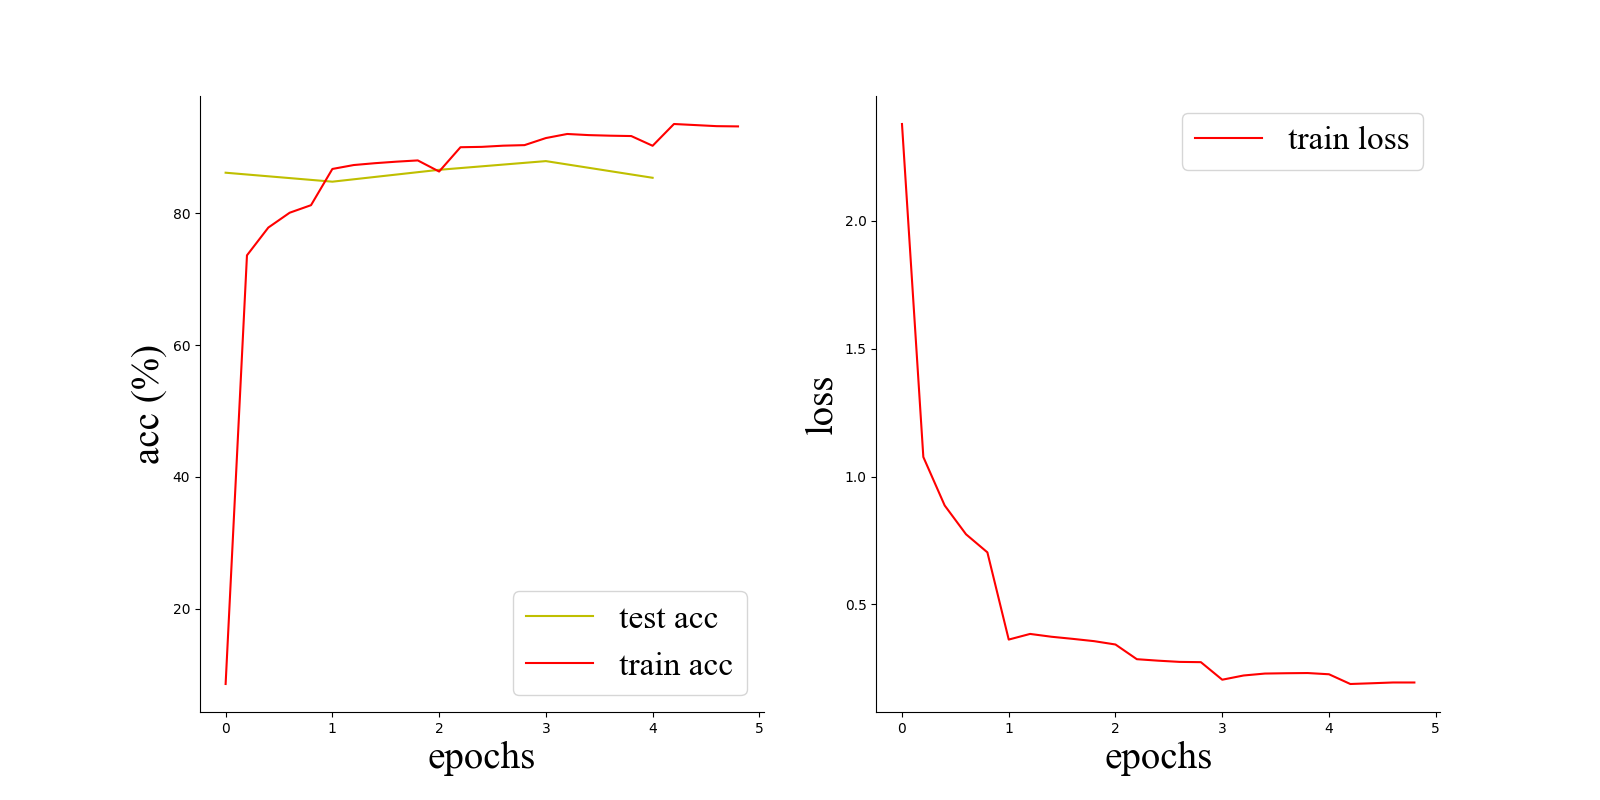
\includegraphics[width=0.8\textwidth]{imgs_5e/AdaDelta.png}
              \caption{AdaDelta的训练结果}
              \label{fig:adadelta}
            \end{figure}         
            最终,经过5个epoch的训练,得到的损失函数值为0.194,训练集和测试集上的准确率分别为0.932和0.854,训练速度为11790.4 examples/sec on cuda:0。\par
        \subsection{Adam}
            自适应矩估计(Adaptive Moment Estimation)\cite{adam},目前最主流的优化方法,比Adadelta多了一项梯度的指数衰减平均(Adadelta是梯度平方的指数衰减平均):
            $$\begin{array}{c}m_t=\beta_1m_{t-1}+(1-\beta_1)g_t\\ v_t=\beta_2v_{t-1}+(1-\beta_2)g_t^2\end{array}$$
            $m_t$和$v_t$分别是$g_t$的第一矩(均值)估计和第二矩(非中心方差)估计;作者注意到了一个问题并给出了解决方案:当两向量初始化为0时,他们在初始或者$\beta_1\text{、}\beta_2$接近于1时偏向于0;他们通过计算经过偏差校正的第一和第二矩估计来抵消偏差:
            \begin{align*}\hat{m}_t&=\frac{m_t}{1-\beta_1^t}\\ \hat{v}_t&=\frac{v_t}{1-\beta_2^t}\end{align*}
            Adam的更新规则如下:
            $$\theta_{t+1}=\theta_t-\dfrac{\eta}{\sqrt{\hat{v}_t}+\epsilon}\hat{m}_t$$
            作者建议设置$\beta_1$为0.9,$\beta_2$为0.999,$\epsilon$为1e-8。\par
            过去的经验表明,Adam算法在实践中表现良好,优于其他自适应学习算法。目前Adam论文在google scholar已经达到了141339的引用数。
            \subsubsection{实现}
            我们需要维护mt,vt两个变量,分别存储梯度的衰减平均与梯度平方的衰减平均,同时在更新时要计算其矩估计,具体更新代码如下:
            \begin{lstlisting}
                mt[:] = beta1 * mt + (1 - beta1) * p2.grad
                vt[:] = beta2 * vt + (1 - beta2) * torch.square(p2.grad)
                mt_hat = mt / (1 - beta1 ** self.t)
                vt_hat = vt / (1 - beta2 ** self.t)
                p2[:] -= p1['lr'] * mt_hat / (torch.sqrt(vt_hat) + epsilon)
            \end{lstlisting}\par
            实验结果如下:
            \begin{figure}[H]
            \centering
                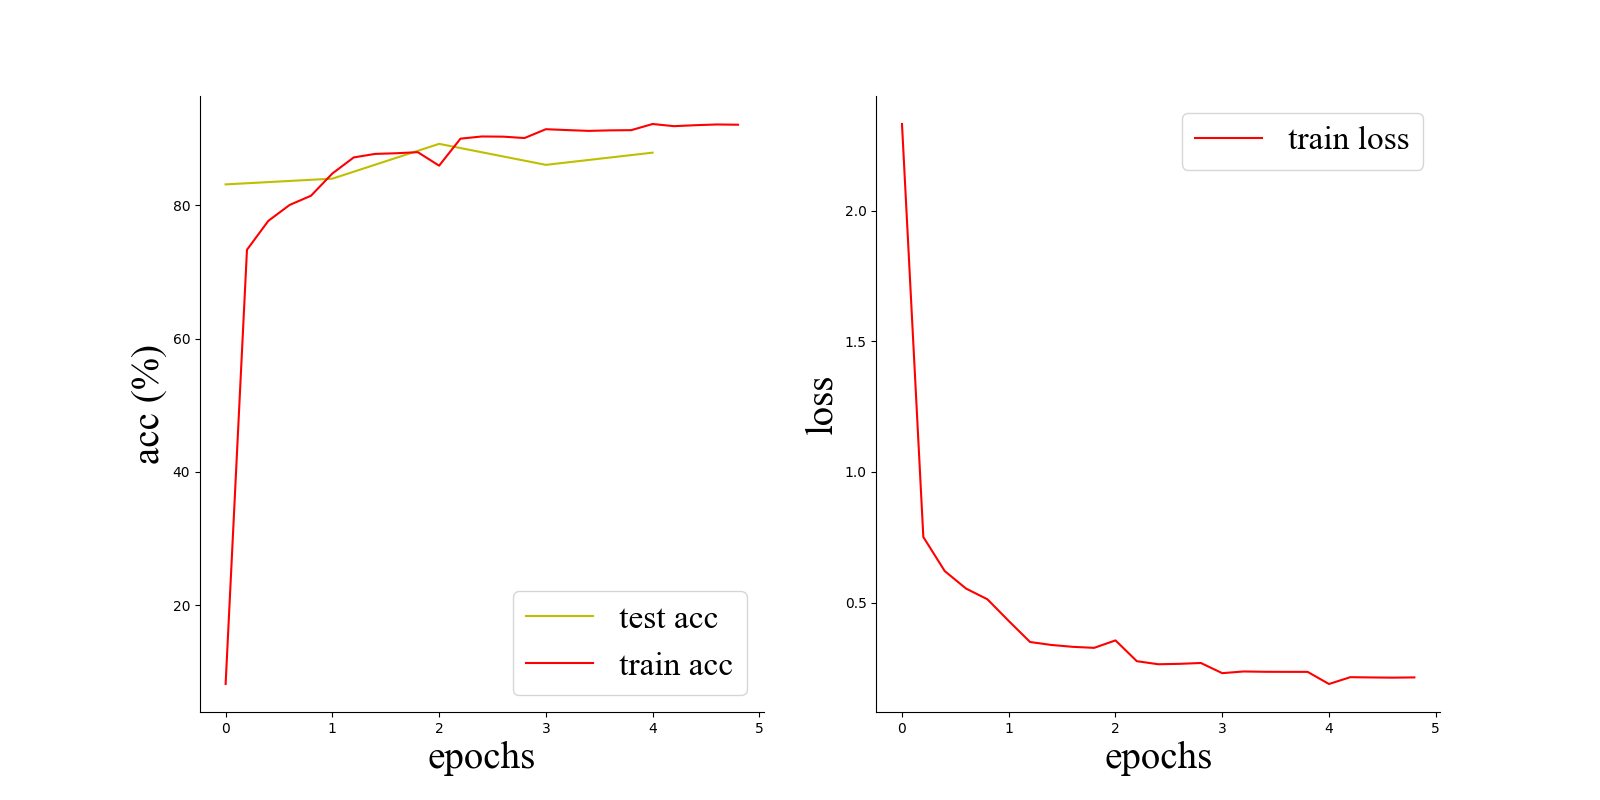
\includegraphics[width=0.8\textwidth]{imgs_5e/Adam.png}
              \caption{Adam的训练结果}
              \label{fig:adam}
            \end{figure}  
            最终,经过5个epoch的训练,得到的损失函数值为0.214,训练集和测试集上的准确率分别为0.921和0.879,训练速度为11817.2 examples/sec on cuda:0。\par
        \subsection{AdaMax}
            在Adam的更新规则中,$v_t$的更新规则为
            $$v_t=\beta_2v_{t-1}+(1-\beta_2)|g_t|^2$$
            AdaMax\cite{adam}将这个更新扩展到了p范数,同时将$\beta_2\text{变成了}\beta_2^p$:
            $$v_t=\beta_2^p v_{t-1}+(1-\beta_2^p)|g_t|^p$$
            p范数通常p的值越大,在数值上会变得越不稳定,这就是为什么“1”和“2”范数在实践中最常见。但是,$∞$范数通常也表现出稳定的行为。为此,作者提出了AdaMax,并证明了$v_t$在$∞$时收敛到以下更稳定的值。为了避免与Adam混淆,我们用$u_t$表示无限范数约束的$v_t$:  
            \begin{align*}u_t=\lim_{p\to\infty}(v_t)^{1/p}&=\lim_{p\to\infty}\left((1-\beta_2^p)\sum_{i=1}^t\beta_2^{p(t-i)}\cdot|g_i|^p\right)^{1/p}\\ &=\lim_{p\to\infty}(1-\beta_2^{p})^{1/p}\left(\sum_{i=1}^t\beta_2^{p(t-i)}\cdot|g_i|^p\right)^{1/p}\\&=\lim_{p\to\infty}\left(\sum_{i=1}^t\left(\beta_2^{(t-i)}\cdot|g_i|\right)^p\right)^{1/p}\\ &=\max\left(\beta_2^{t-1}|g_1|,\beta_2^{t-2}|g_2|,\ldots,\beta_2|g_{t-1}|,|g_t|\right)\end{align*}
            简写为
            $$u_t=\max(\beta_2\cdot u_{t-1},|g_t|)$$
            更新方式变为了
            $$\theta_{t+1}=\theta_t-\dfrac{\eta}{u_t}\hat{m}_t$$
            $u_t$不需要偏差校正,因为他依赖于max运算,不会很容易偏向0. 其余参数与Adam类似。
            \subsubsection{实现}
            注意到更新方式中的max为元素级的函数,即对两个张量的每个元素作比较,留下较大者,在实现中我们先将两个需要比较的张量concat到一个张量内后利用torch的amax函数实现(参考torch源码):
            \begin{lstlisting}
                mt[:] = beta1 * mt + (1 - beta1) * p2.grad
                temp = torch.cat([(beta2 * ut).unsqueeze(0), (p2.grad.abs() + epsilon).unsqueeze(0)], 0)
                ut[:] = torch.amax(temp, 0, keepdim=False)
                mt_hat = mt / (1 - beta1 ** self.t)
                p2[:] -= p1['lr'] * mt_hat / ut
            \end{lstlisting}\par
            实验结果为
            \begin{figure}[H]
                \centering
                    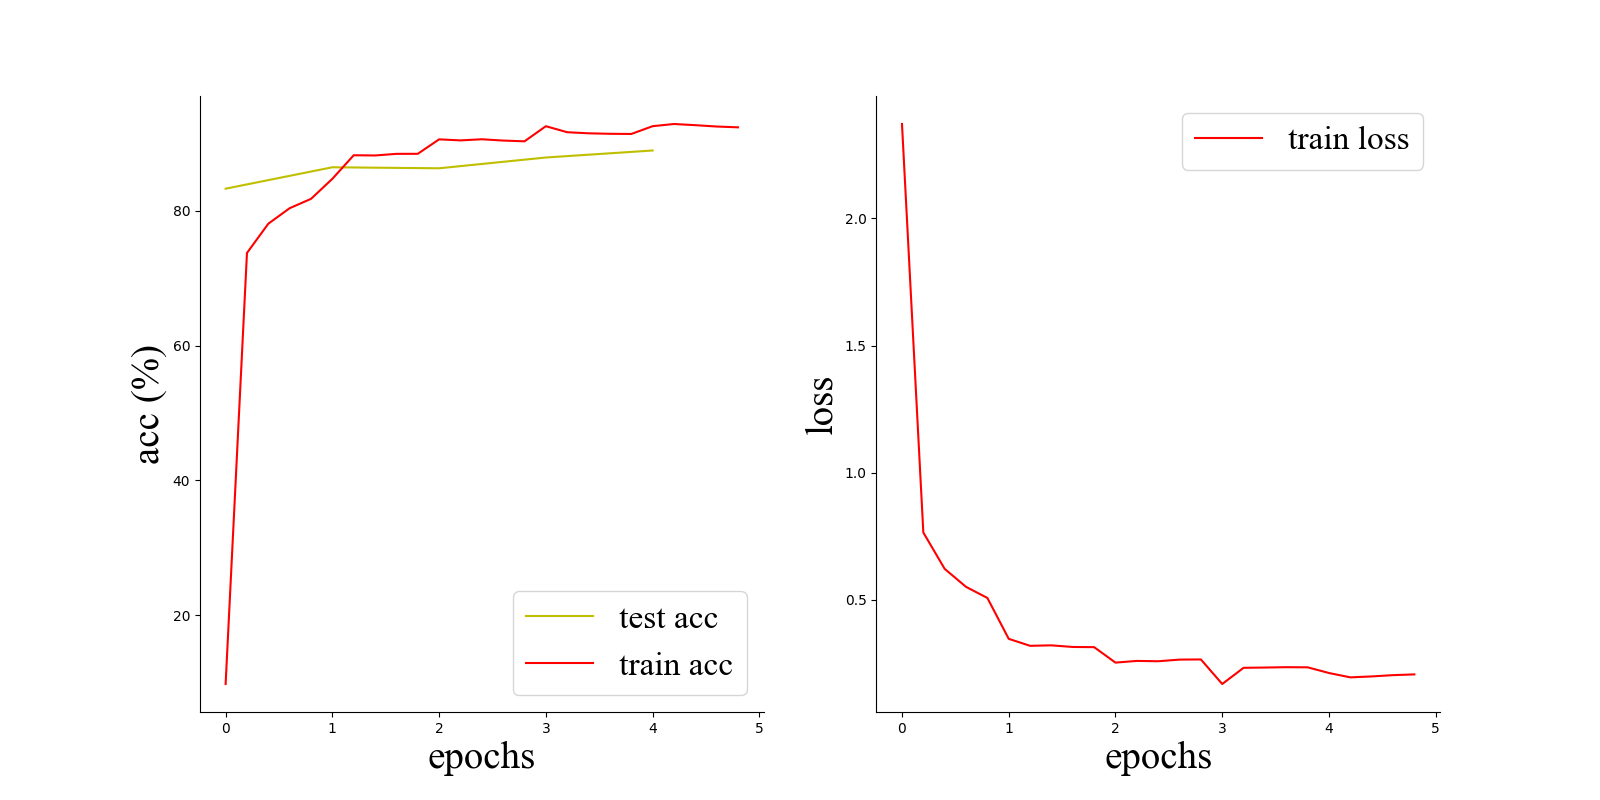
\includegraphics[width=0.8\textwidth]{imgs_5e/AdaMax.png}
                  \caption{AdaMax的训练结果}
                  \label{fig:adamax}
            \end{figure}  
             最终,经过5个epoch的训练,得到的损失函数值为0.206,训练集和测试集上的准确率分别为0.924和0.890,训练速度为11917.8 examples/sec on cuda:0。\par
        \subsection{NAdam}
            Adam可以被视为是RMSprop与momentum的组合,即梯度平方衰减平均+梯度衰减平军;之前提到Nesterov加速梯度性能上是优于momentum的;基于此提出了Nadam\cite{nadam},融合Adam与NAG。\par
            注意到NAG需要修改梯度的计算,因此我们需要调整Adam的动量项$m_t$,注意到之前SGD with momentum的NAG优化中,更新规则为:  
            \begin{align*}
                g_t&=\nabla_{\theta_t}J(\theta_t-\gamma m_{t-1})\\ m_t&=\gamma m_{t-1}+\eta g_t\\ \theta_{t+1}&=\theta_t-m_t
            \end{align*}
            该更新规则中,动量项m被应用了两次,一次计算梯度,一次更新参数;Nadam将其简化为一次,使用当前时间步的m直接更新参数,具体见下述更新规则:\begin{align*}g_t&=\nabla_{\theta_t}J(\theta_t)\\ m_t&=\gamma m_{t-1}+\eta g_t\\ \theta_{t+1}&=\theta_t-(\gamma m_t+\eta g_t)\end{align*}
            对比SGD with momentum的更新:$\theta_{t+1}=\theta_t-(\gamma m_{t-1}+\eta g_t)$,可以发现仅仅是$m_t \text{与}m_{t-1}$的差别,我们首先给出Adam的更新规则(已将动量项更新代入)
            \begin{align*}
            \theta_{t+1}&=\theta_t-\dfrac{\eta}{\sqrt{\hat{v}_t}+\epsilon}(\dfrac{\beta_1m_{t-1}}{1-\beta_1^t}+\dfrac{(1-\beta_1)g_t}{1-\beta_1^t})\\
            &=\theta_{t}-\frac{\eta}{\sqrt{\hat{v}_{t}}+\epsilon}(\beta_{1}\hat{m}_{t-1}+\frac{(1-\beta_{1})g_{t}}{1-\beta_{1}^{t}})
            \end{align*}
            该方程与动量SGD的更新公式十分相似,我们现在做一样的事情(即把$m_{t-1}\text{代换为}m_t$,即得出Nadam的更新规则:
            $$\theta_{t+1}=\theta_t-\dfrac{\eta}{\sqrt{\hat{v}_t}+\epsilon}(\beta_1\hat{m}_t+\dfrac{(1-\beta_1)g_t}{1-\beta_1^t})$$
            \subsubsection{实现}
            由于最终给出的更新规则十分清晰,因此我们在Adam的基础之上修改最终的更新代码即可,具体地说,更新的关键代码如下:
            \begin{lstlisting}
                mt[:] = beta1 * mt + (1 - beta1) * p2.grad
                vt[:] = beta2 * vt + (1 - beta2) * torch.square(p2.grad)
                mt_hat = mt / (1 - beta1 ** self.t)
                vt_hat = vt / (1 - beta2 ** self.t)
                p2[:] -= p1['lr'] * (beta1 * mt_hat + (1 - beta1) * p2.grad) / (1 - beta1 ** self.t) / (torch.sqrt(vt_hat) + epsilon)
            \end{lstlisting}\par
            实验结果如下:
            \begin{figure}[H]
                \centering
                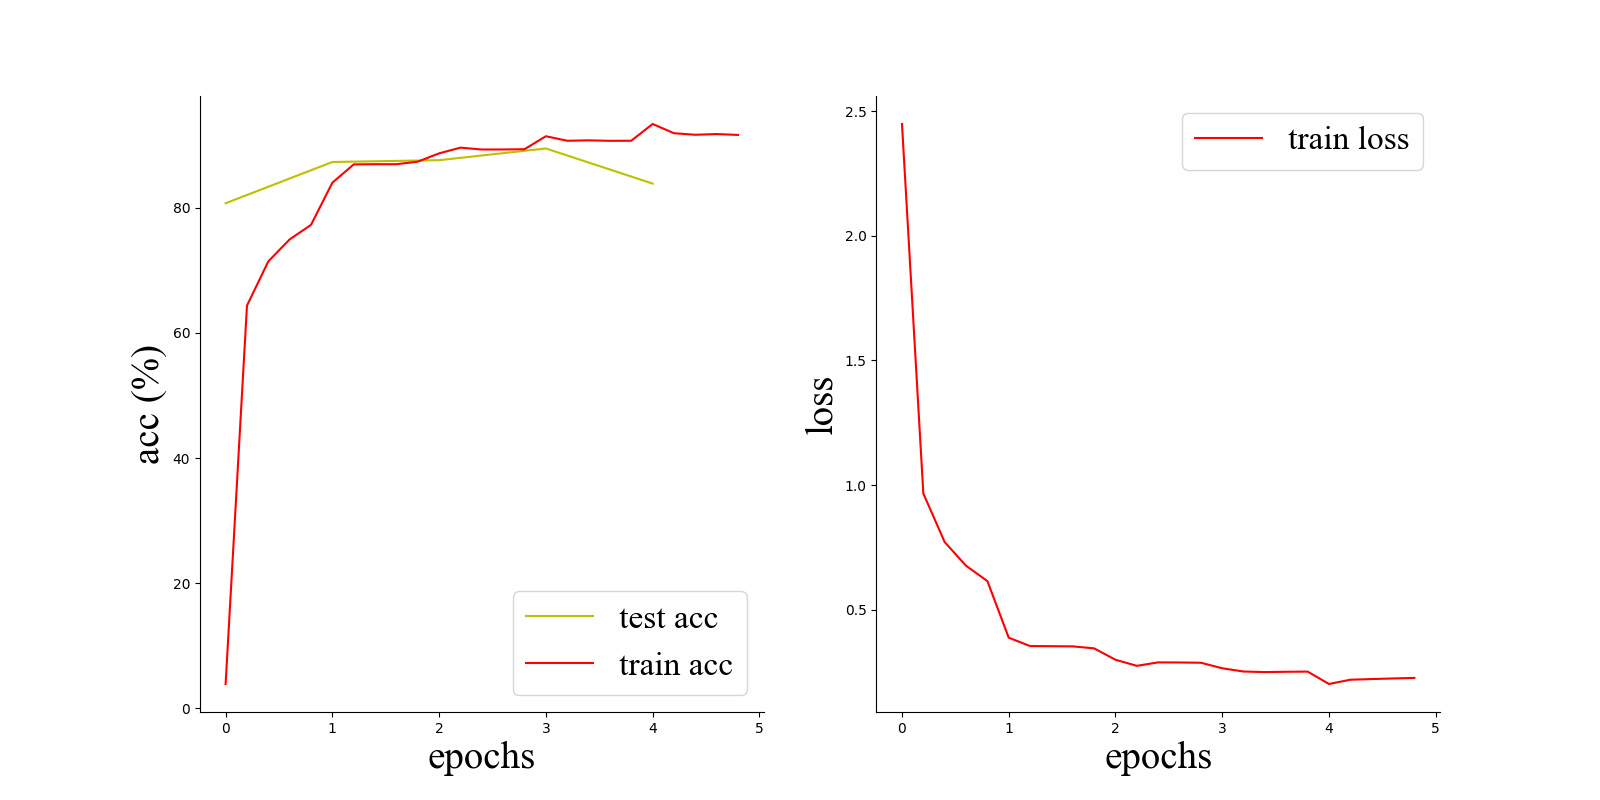
\includegraphics[width=0.8\textwidth]{imgs_5e/NAdam.png}
                  \caption{NAdam的训练结果}
                  \label{fig:nadam}
            \end{figure}  
             最终,经过5个epoch的训练,得到的损失函数值为0.227,训练集和测试集上的准确率分别为0.916和0.838,训练速度为11465.5 examples/sec on cuda:0。\par
\newpage
\bibliographystyle{plain}
\bibliography{my}
\newpage
\section{附录}
            \begin{figure}[H]
                    \centering
        	\begin{minipage}{0.48\textwidth}
        		\centering
        		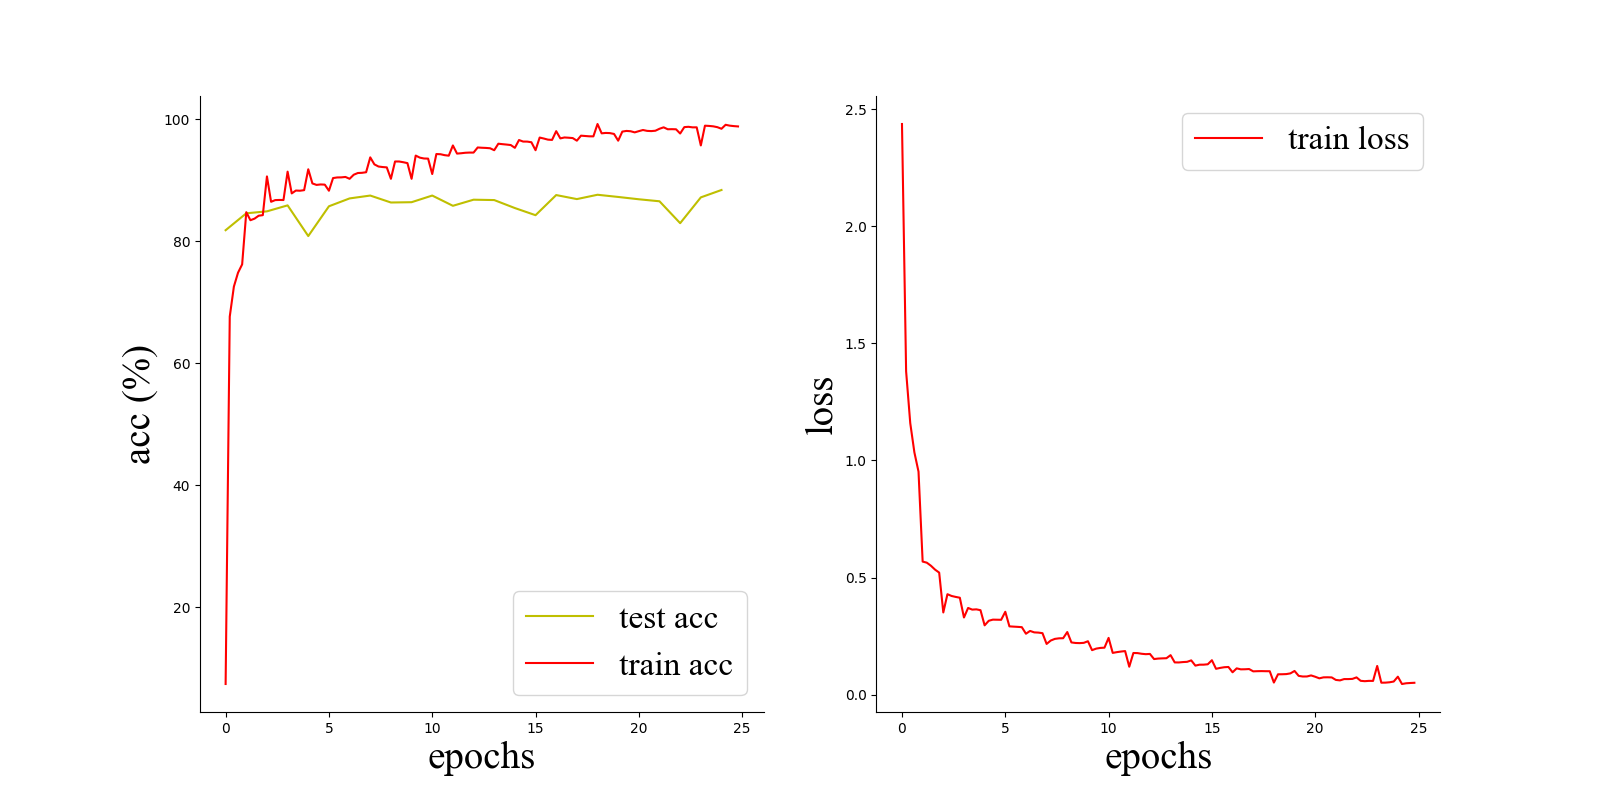
\includegraphics[width=0.83\textwidth]{imgs_25e/SGD.png}
        		\caption{\fontsize{10pt}{15pt}\selectfont SGD的训练结果 25epochs}
        	\end{minipage}
        	\hspace{0cm}% 图片间距
        	\hfill% 撑满整行
        	\begin{minipage}{0.48\textwidth}
        		\centering
        		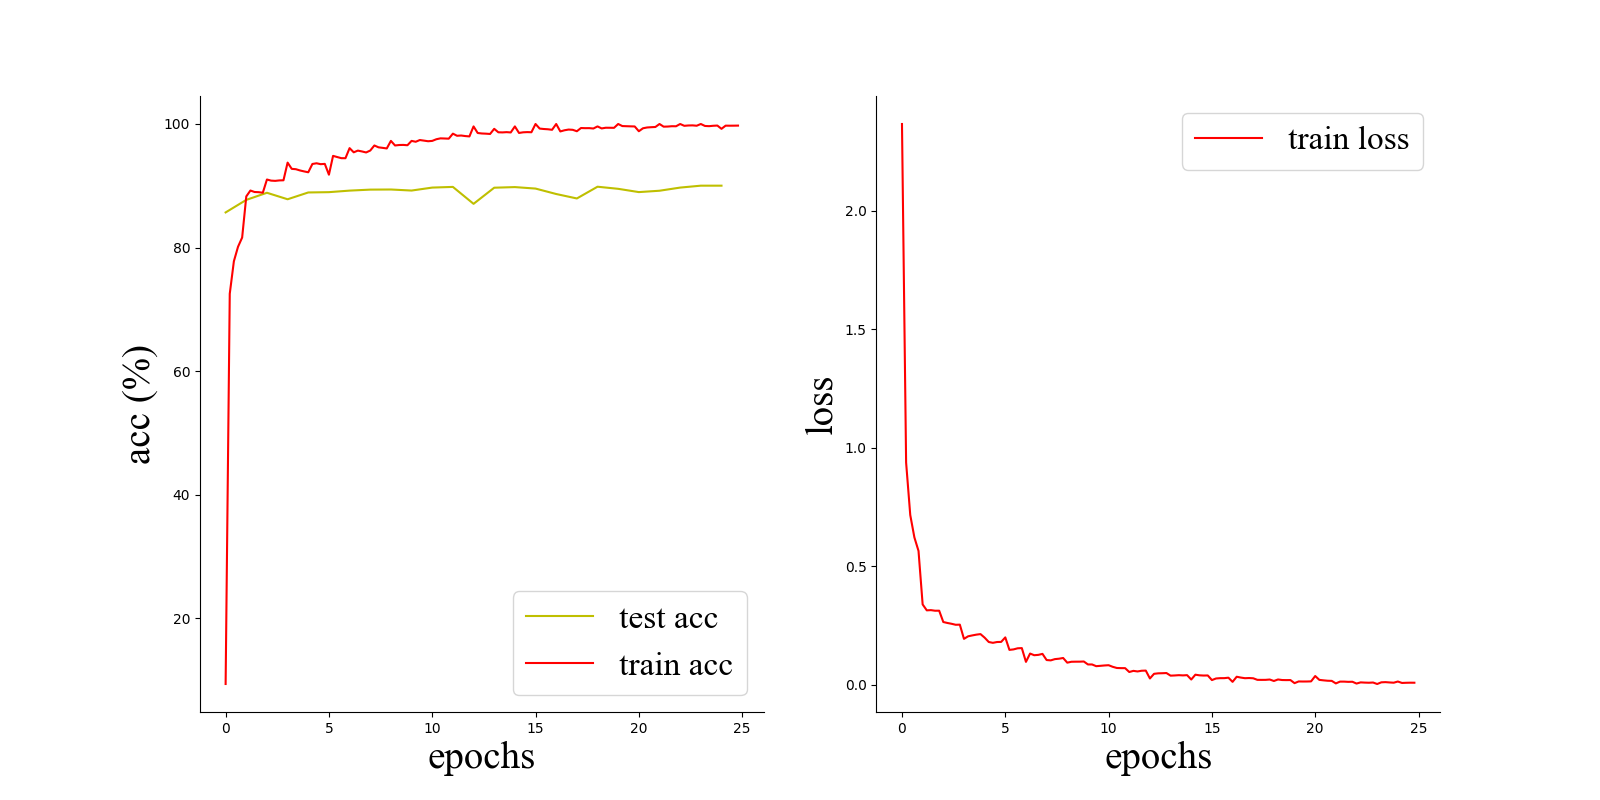
\includegraphics[width=0.83\textwidth]{imgs_25e/SGD_momentum.png}
        		\caption{\fontsize{10pt}{15pt}\selectfont SGD\_momentum的训练结果 25epochs}
        	\end{minipage}
            \end{figure}    
            \begin{figure}[H]
                    \centering
        	\begin{minipage}{0.48\textwidth}
        		\centering
        		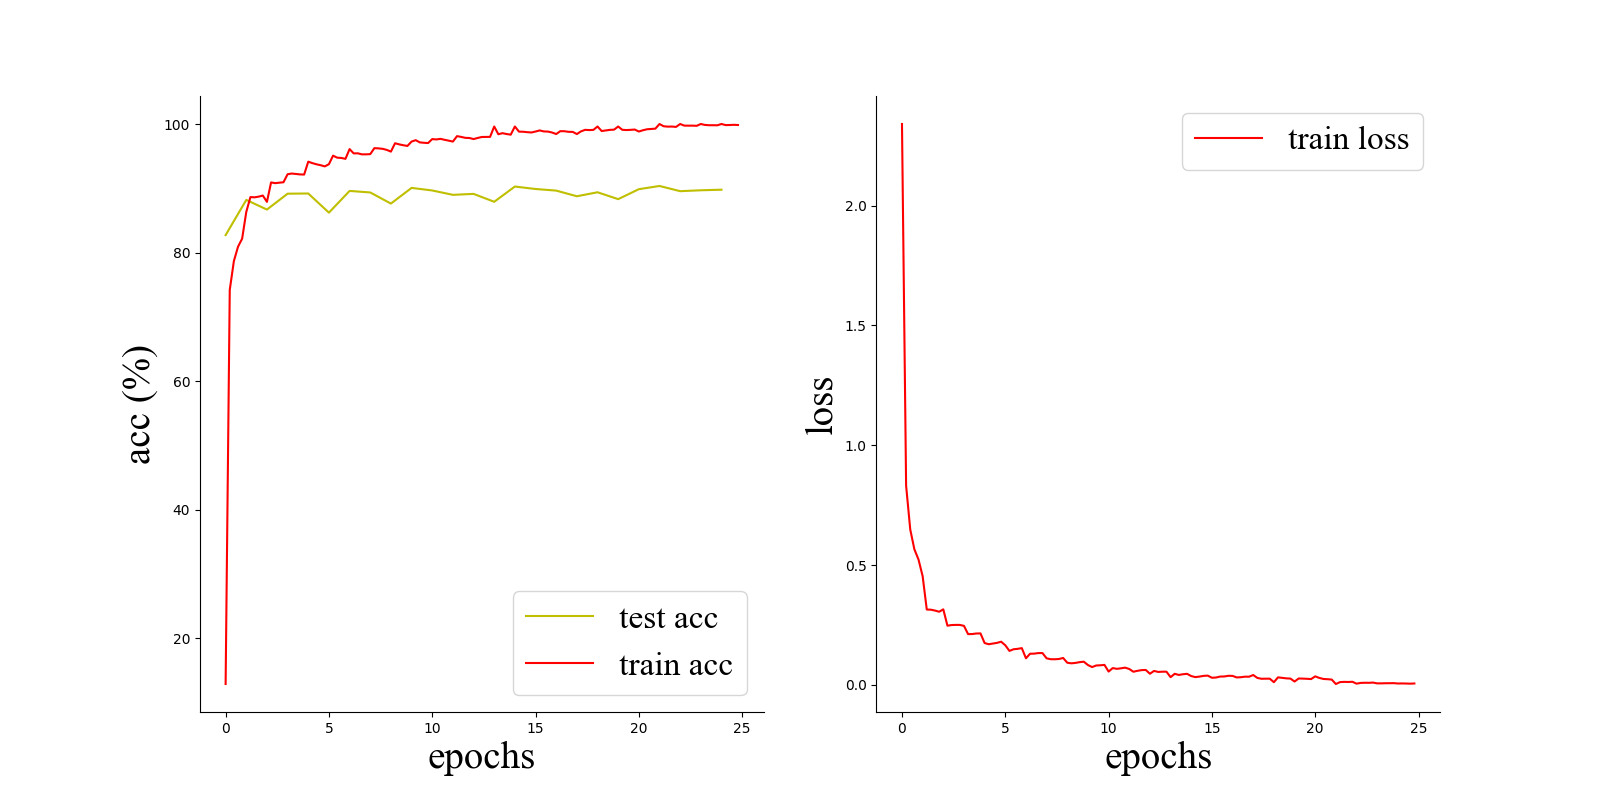
\includegraphics[width=0.83\textwidth]{imgs_25e/SGD_momentum_nesterov.png}
        		\caption{\fontsize{10pt}{15pt}\selectfont SGD\_momentum\_nesterov的训练结果 25epochs}
        	\end{minipage}
        	\hspace{0cm}% 图片间距
        	\hfill% 撑满整行
        	\begin{minipage}{0.48\textwidth}
        		\centering
        		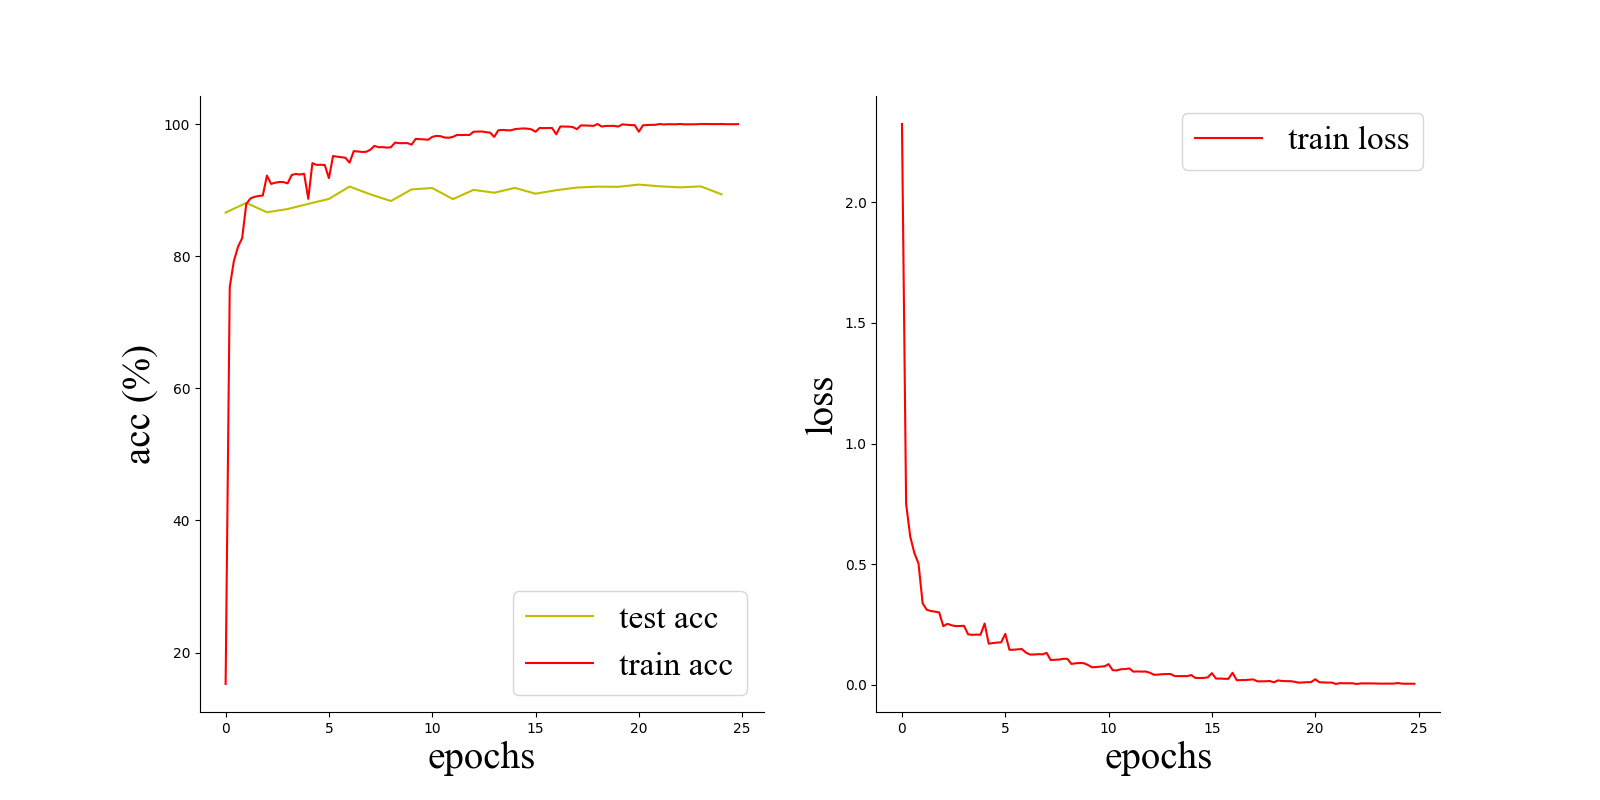
\includegraphics[width=0.83\textwidth]{imgs_25e/AdaGrad.png}
        		\caption{\fontsize{10pt}{15pt}\selectfont AdaGrad\_momentum的训练结果 25epochs}
        	\end{minipage}
            \end{figure}  
            \begin{figure}[H]
                    \centering
        	\begin{minipage}{0.48\textwidth}
        		\centering
        		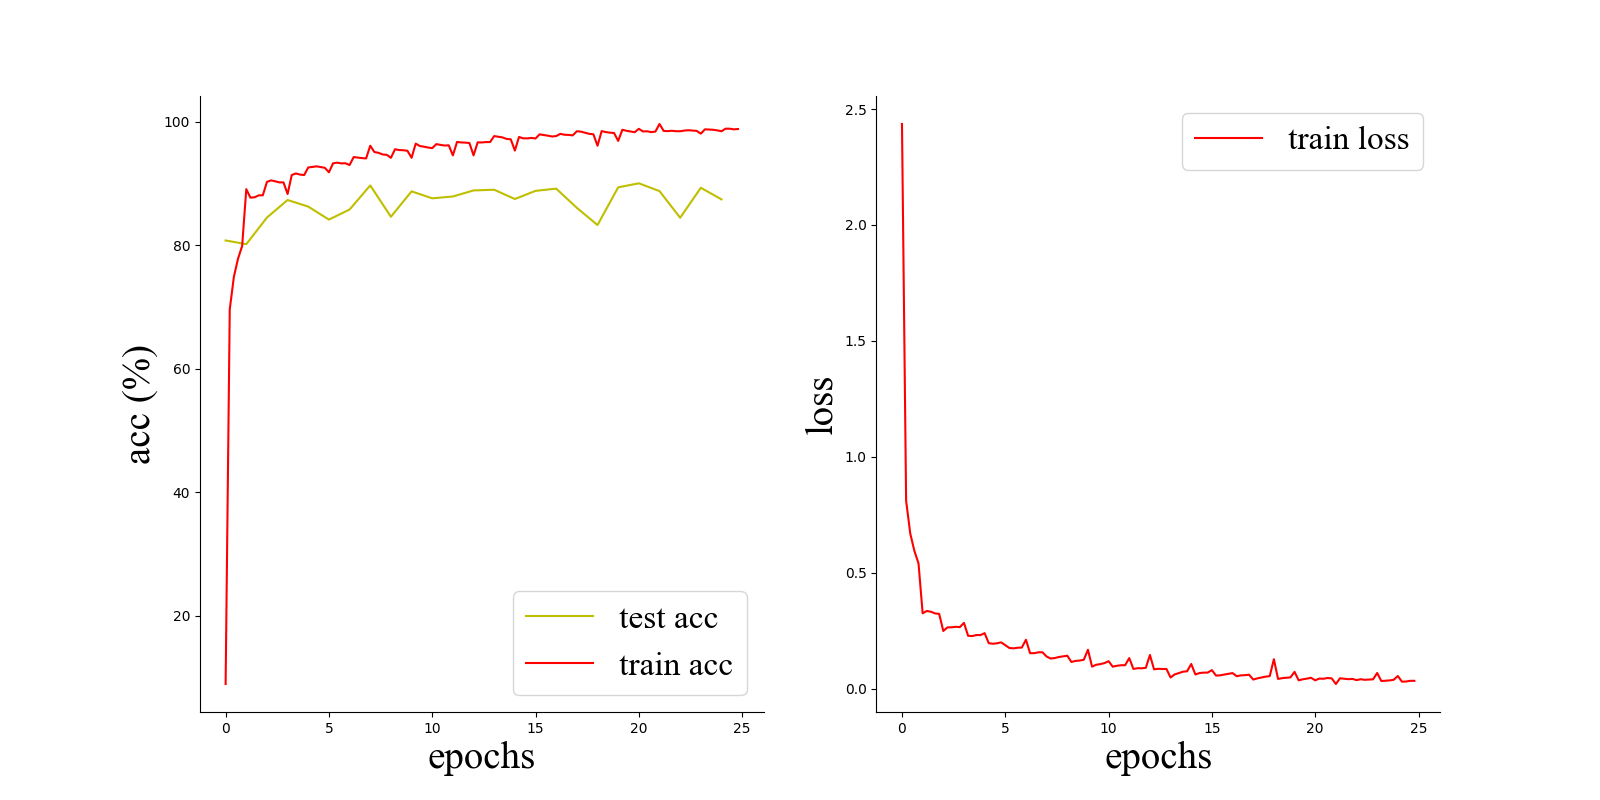
\includegraphics[width=0.83\textwidth]{imgs_25e/RMSProp.png}
        		\caption{\fontsize{10pt}{15pt}\selectfont RMSProp的训练结果 25epochs}
        	\end{minipage}
        	\hspace{0cm}% 图片间距
        	\hfill% 撑满整行
        	\begin{minipage}{0.48\textwidth}
        		\centering
        		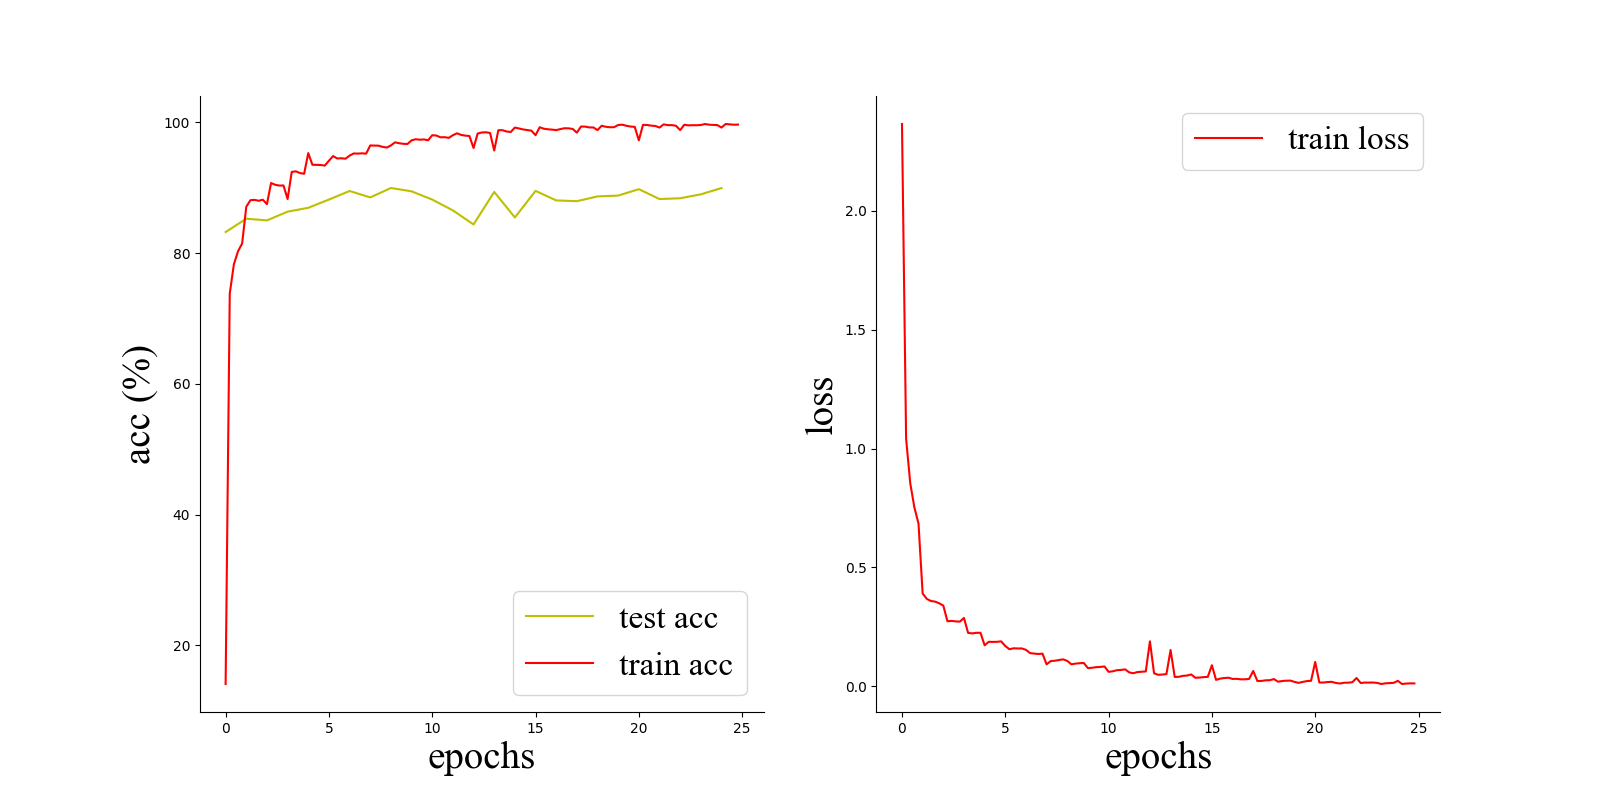
\includegraphics[width=0.83\textwidth]{imgs_25e/Adadelta.png}
        		\caption{\fontsize{10pt}{15pt}\selectfont Adadelta的训练结果 25epochs}
        	\end{minipage}
            \end{figure}  
            \begin{figure}[H]
                    \centering
        	\begin{minipage}{0.48\textwidth}
        		\centering
        		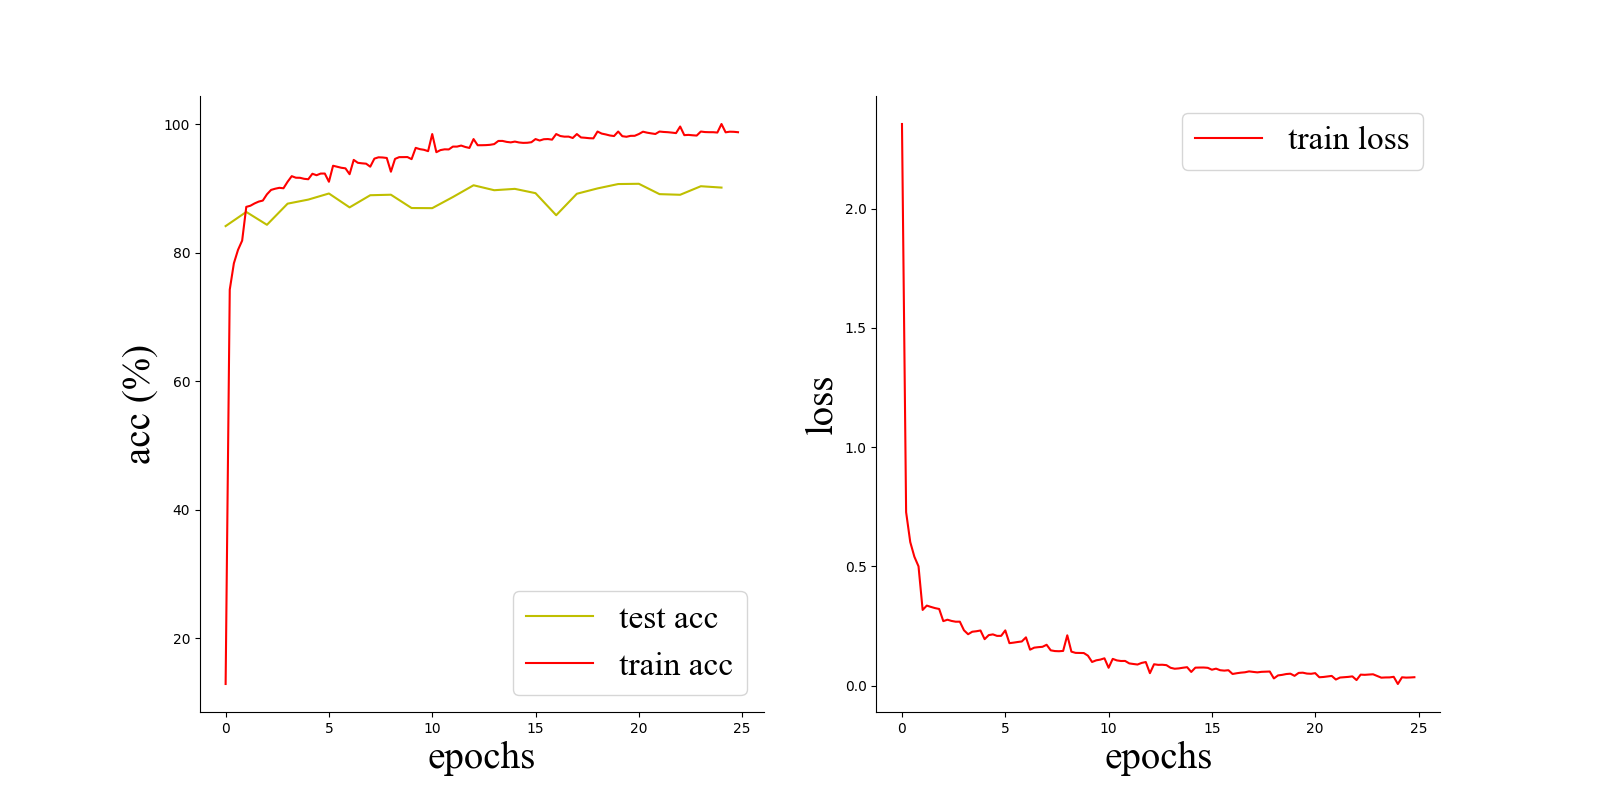
\includegraphics[width=0.83\textwidth]{imgs_25e/adam.png}
        		\caption{\fontsize{10pt}{15pt}\selectfont Adam的训练结果 25epochs}
        	\end{minipage}
        	\hspace{0cm}% 图片间距
        	\hfill% 撑满整行
        	\begin{minipage}{0.48\textwidth}
        		\centering
        		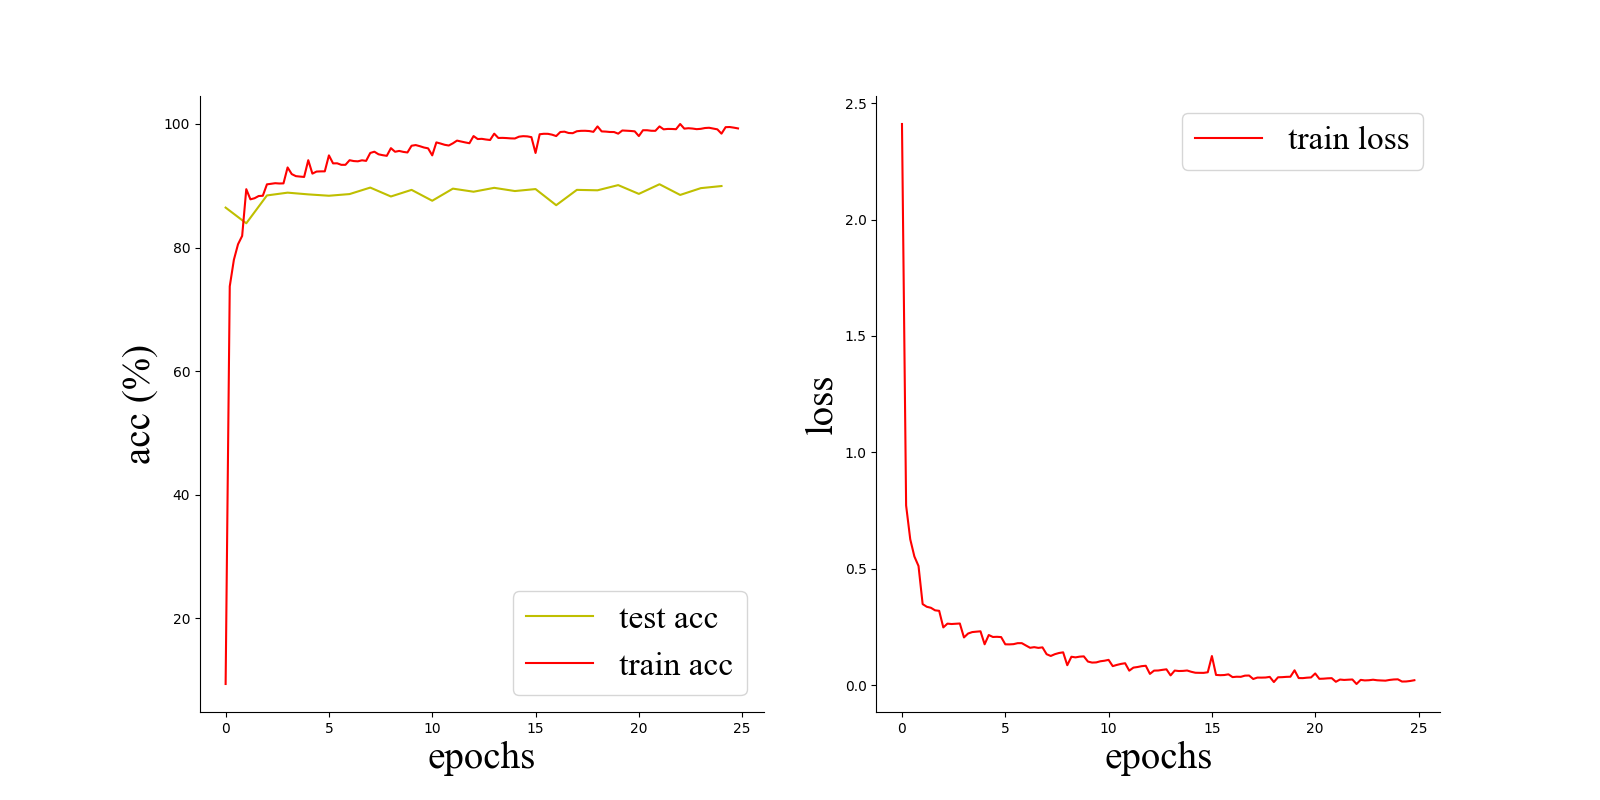
\includegraphics[width=0.83\textwidth]{imgs_25e/AdaMax.png}
        		\caption{\fontsize{10pt}{15pt}\selectfont AdaMax的训练结果 25epochs}
        	\end{minipage}
            \end{figure}  
            \begin{figure}[H]
                    \centering
        	\begin{minipage}{0.48\textwidth}
                    \centering
        		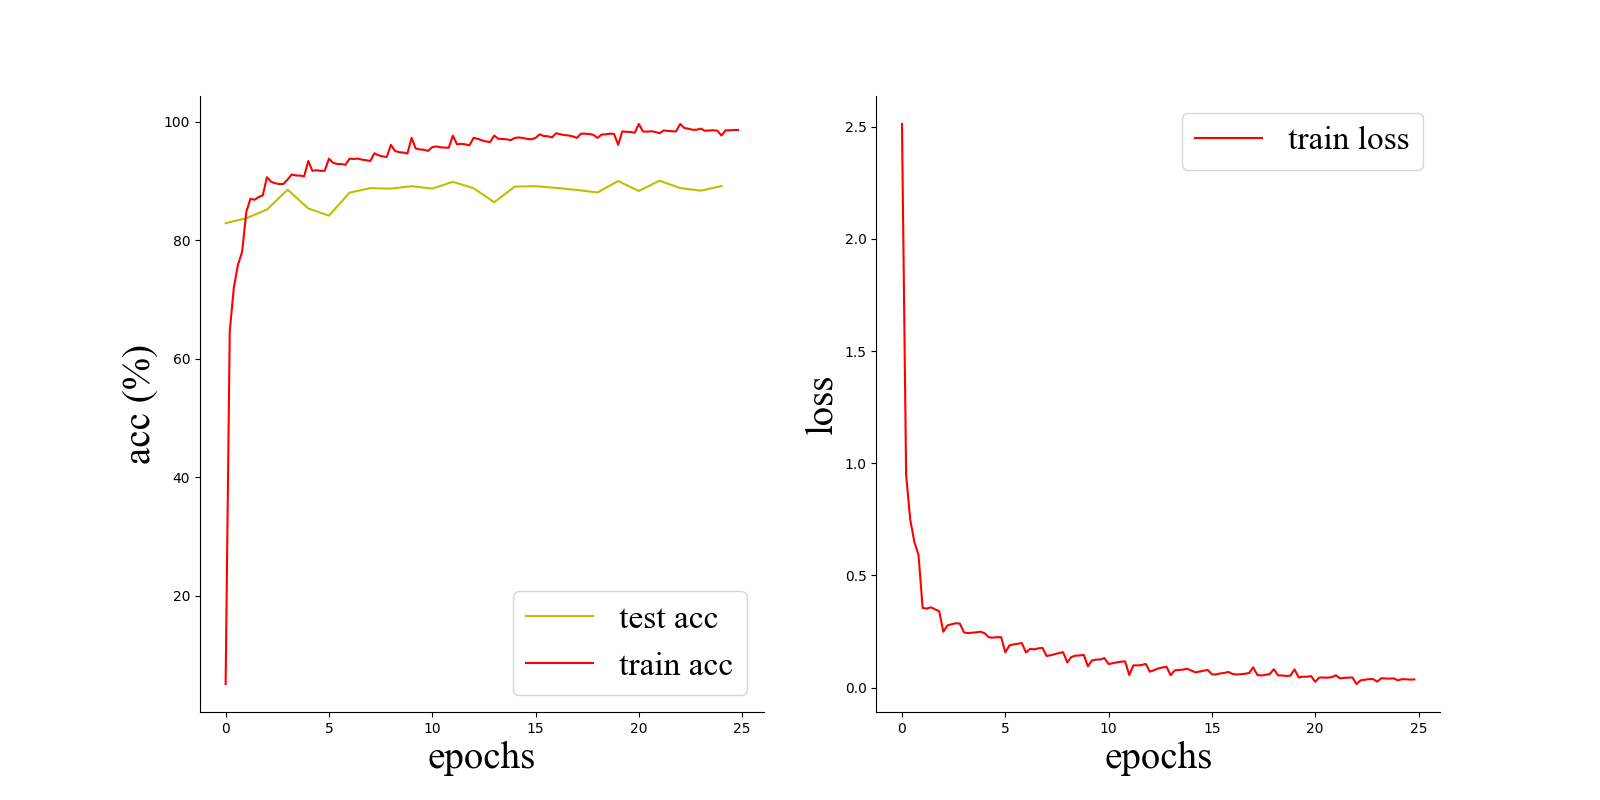
\includegraphics[width=0.83\textwidth]{imgs_25e/nadam.png}
        		\caption{\fontsize{10pt}{15pt}\selectfont NAdam的训练结果 25epochs}
        	\end{minipage}
            \end{figure}               
\end{document}% 结束文档编辑,后面写啥都编译不出来
